\documentclass[11pt,a4paper]{article}
\usepackage[margin=1in]{geometry}
\usepackage{graphicx}
\usepackage{booktabs}
\usepackage{longtable}
\usepackage{hyperref}
\usepackage{xcolor}
\usepackage{float}
\usepackage[font=small]{caption}
\usepackage{seqsplit}
\usepackage{array}
\usepackage{tabularx}

\hypersetup{
  colorlinks=true,
  linkcolor=blue!60!black,
  urlcolor=blue!60!black,
  citecolor=blue!60!black
}

\title{\textbf{RBX1 De Novo Binder Design}\\[4pt]Campaign Report}
\author{Sergio E. Mares}
\date{March 23, 2026}

\begin{document}
\maketitle
\tableofcontents
\newpage

%% ============================================================
\section{Executive Summary}
%% ============================================================

This report documents a large-scale de novo binder design campaign targeting the human RBX1 RING-H2 domain. Key outcomes:

\begin{itemize}
  \item \textbf{20,724} unique binder designs were generated and scored with Boltz-2.
  \item \textbf{60} designs were validated with AlphaFold3 (AF3); \textbf{14} achieved AF3 ipTM $\geq 0.70$ (``top hits'').
  \item \textbf{$\sim$1,225} designs were validated with OpenFold3 (OF3).
  \item \textbf{81} designs were submitted to the ADAPTYV Boltz-2 competition and independently re-scored; \textbf{33} survived (competition ipSAE $\geq 0.6$).
  \item \textbf{Key finding:} Boltz-2 pipeline scores (ipSAE, ipTM) do \emph{not} predict AF3 validation ($r \approx 0.08$ for ipTM, $r = -0.044$ for ipSAE) or competition outcomes ($r \approx 0.31$ for ipSAE).
  \item \textbf{Best overall design:} \texttt{w2\_design\_1209} --- AF3 ipTM = 0.77, competition Pb ipSAE = 0.81, OF3 ipTM = 0.75.
\end{itemize}

%% ============================================================
\section{Target: RBX1}
%% ============================================================

RBX1 (RING-Box protein 1, PDB: 5H0P) is a 108-amino-acid RING-H2 domain that coordinates three zinc ions and serves as the catalytic subunit of Cullin--RING E3 ubiquitin ligase complexes. The target presents two distinct binding interfaces:

\begin{itemize}
  \item \textbf{E2 face} ($\sim$35 interface residues): the surface that recruits E2 ubiquitin-conjugating enzymes. This face was the primary design target, targeted with enhanced hotspot sets derived from DMS data.
  \item \textbf{Cullin face} ($\sim$31 interface residues): the surface that contacts the Cullin scaffold protein.
\end{itemize}

A 165-sequence multiple sequence alignment (MSA) was used for evolutionary conservation analysis. Zinc-coordinating cysteines and histidines are absolutely conserved and dominate ESM-2 deep mutational scanning (DMS) sensitivity profiles.

%% ============================================================
\section{Design Pipeline}
%% ============================================================

Two complementary pipelines were employed:

\begin{enumerate}
  \item \textbf{RFdiffusion $\rightarrow$ ProteinMPNN $\rightarrow$ Boltz-2}: The primary pipeline. RFdiffusion generates backbone scaffolds conditioned on target hotspot residues; ProteinMPNN designs sequences; Boltz-2 scores complexes with MSA input.
  \item \textbf{BoltzGen}: An alternative generative pipeline that directly samples binder sequences and structures.
\end{enumerate}

Hotspot configurations included:
\begin{itemize}
  \item \textbf{E2 Enhanced} (+DMS-derived contacts): the majority of E2-face designs.
  \item \textbf{E2 Standard}: canonical E2-face hotspots.
  \item \textbf{Cullin}: Cullin-face hotspots.
\end{itemize}

\begin{table}[H]
\centering
\caption{Campaign breakdown by target face.}
\label{tab:campaigns}
\begin{tabular}{lrrr}
\toprule
\textbf{Campaign} & \textbf{Designs} & \textbf{Mean ipSAE} & \textbf{AF3-validated} \\
\midrule
E2 Face     & 12,112 & 0.227 & 45 \\
Cullin Face &  6,791 & 0.205 &  6 \\
BoltzGen    &  1,820 & 0.446 &  9 \\
\midrule
\textbf{Total} & \textbf{20,723} & --- & \textbf{60} \\
\bottomrule
\end{tabular}
\end{table}

%% ============================================================
\section{Scoring and Validation}
%% ============================================================

Designs were evaluated at four levels of increasing cost and reliability:

\begin{enumerate}
  \item \textbf{Boltz-2 (primary scoring):} All 20,724 designs scored using Boltz-2 with target MSA. Metrics: ipTM, pTM, pLDDT, ipSAE.
  \item \textbf{OpenFold3 (secondary validation):} $\sim$1,225 top designs validated. OF3 provides an independent structure prediction check.
  \item \textbf{AlphaFold3 (ground truth):} 60 designs validated via the AF3 web server. AF3 ipTM $\geq 0.70$ is considered a ``top hit.''
  \item \textbf{ADAPTYV Competition (Pb):} 81 designs submitted and independently re-scored by competition organizers using a fine-tuned Boltz-2 setup. Survival threshold: ipSAE $\geq 0.6$.
\end{enumerate}

%% ============================================================
\section{Cross-Validation Analysis}
%% ============================================================

A central finding of this campaign is that \textbf{Boltz-2 pipeline metrics do not predict AF3 or competition outcomes}. This section presents the key correlation analyses.

\subsection{ipSAE vs.\ AF3 ipTM}

\begin{figure}[H]
\centering
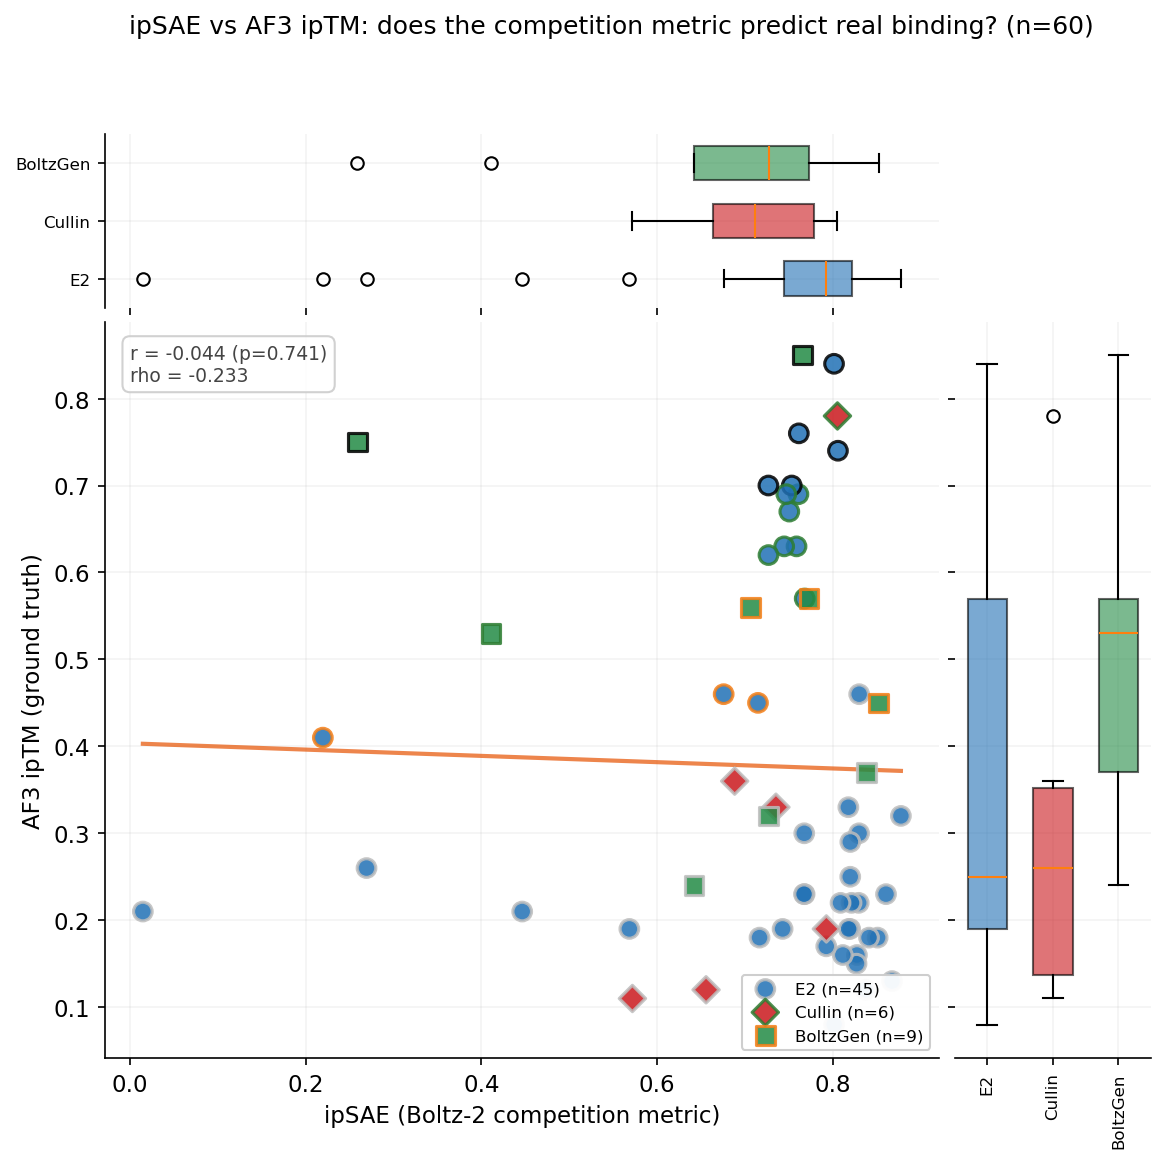
\includegraphics[width=0.85\textwidth]{rbx1_plots/pipe_ipsae_vs_af3.png}
\caption{Boltz-2 ipSAE vs.\ AlphaFold3 ipTM for 60 validated designs. Pearson $r = -0.044$. The competition ranking metric does not predict real binding as assessed by AF3.}
\label{fig:ipsae_vs_af3}
\end{figure}

\subsection{Boltz-2 ipTM vs.\ AF3 ipTM}

\begin{figure}[H]
\centering
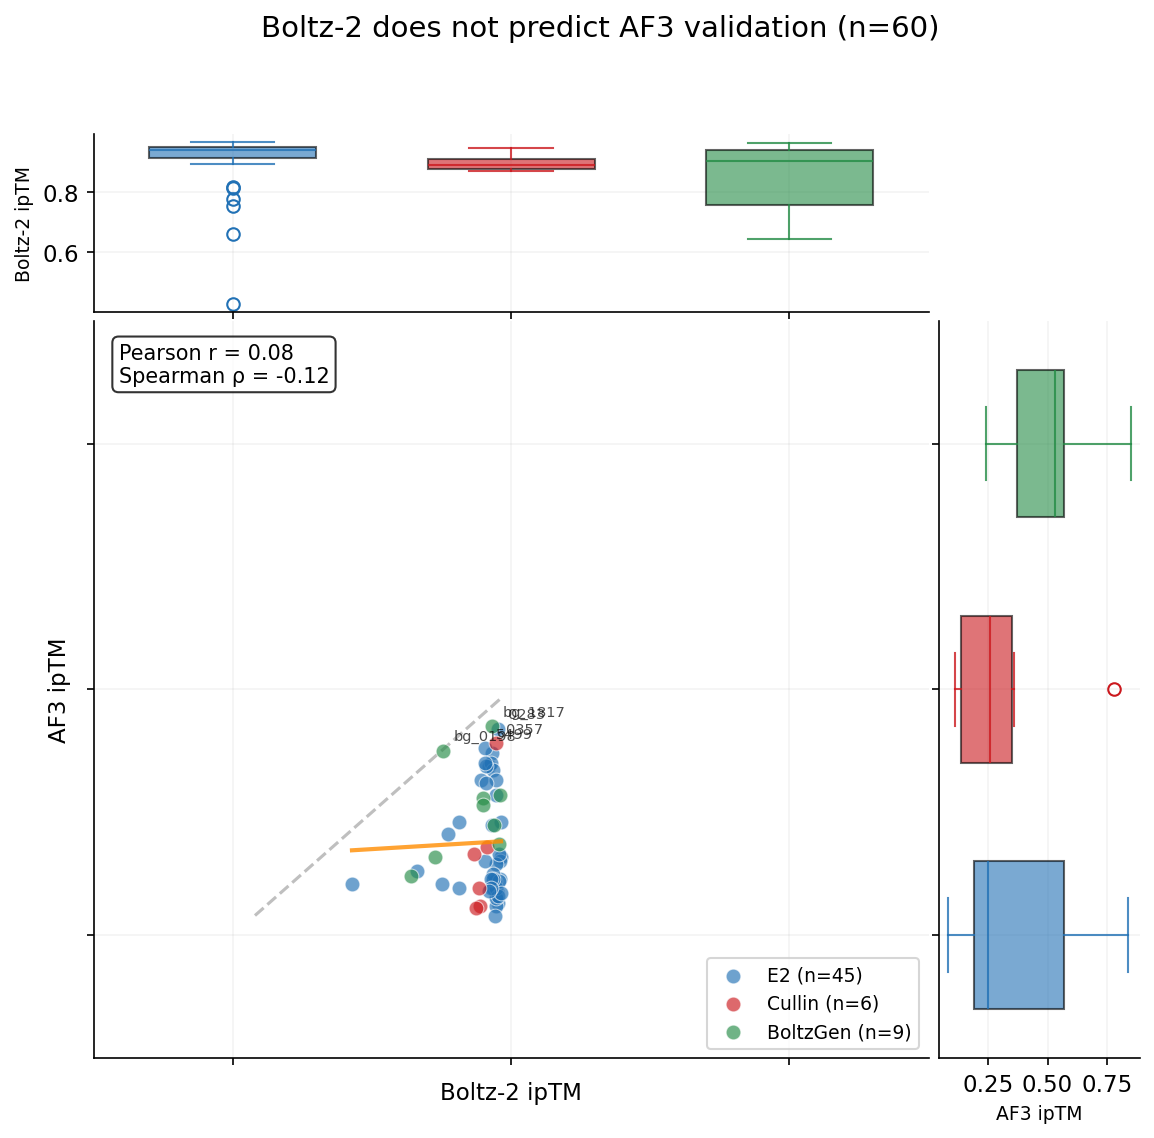
\includegraphics[width=0.85\textwidth]{rbx1_plots/pipe_boltz_vs_af3.png}
\caption{Boltz-2 ipTM vs.\ AlphaFold3 ipTM ($n = 60$). Pearson $r = 0.08$, Spearman $\rho = -0.12$. No predictive relationship.}
\label{fig:boltz_vs_af3}
\end{figure}

\subsection{AF3 vs.\ OF3}

\begin{figure}[H]
\centering
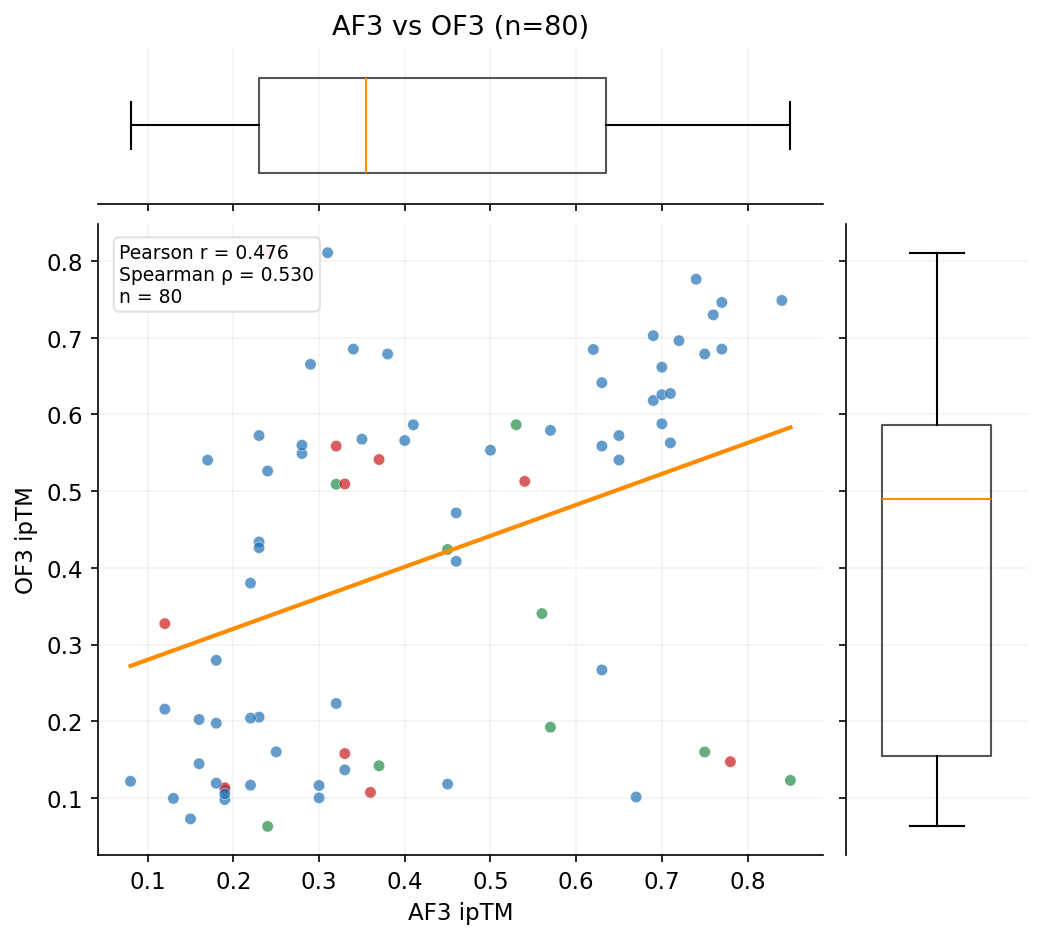
\includegraphics[width=0.85\textwidth]{rbx1_plots/pipe_af3_vs_of3.png}
\caption{AlphaFold3 ipTM vs.\ OpenFold3 ipTM for 49 designs with both scores. Pearson $r = 0.57$, Spearman $\rho = 0.49$. Moderate positive correlation.}
\label{fig:af3_vs_of3}
\end{figure}

\subsection{Boltz-2 vs.\ OF3}

\begin{figure}[H]
\centering
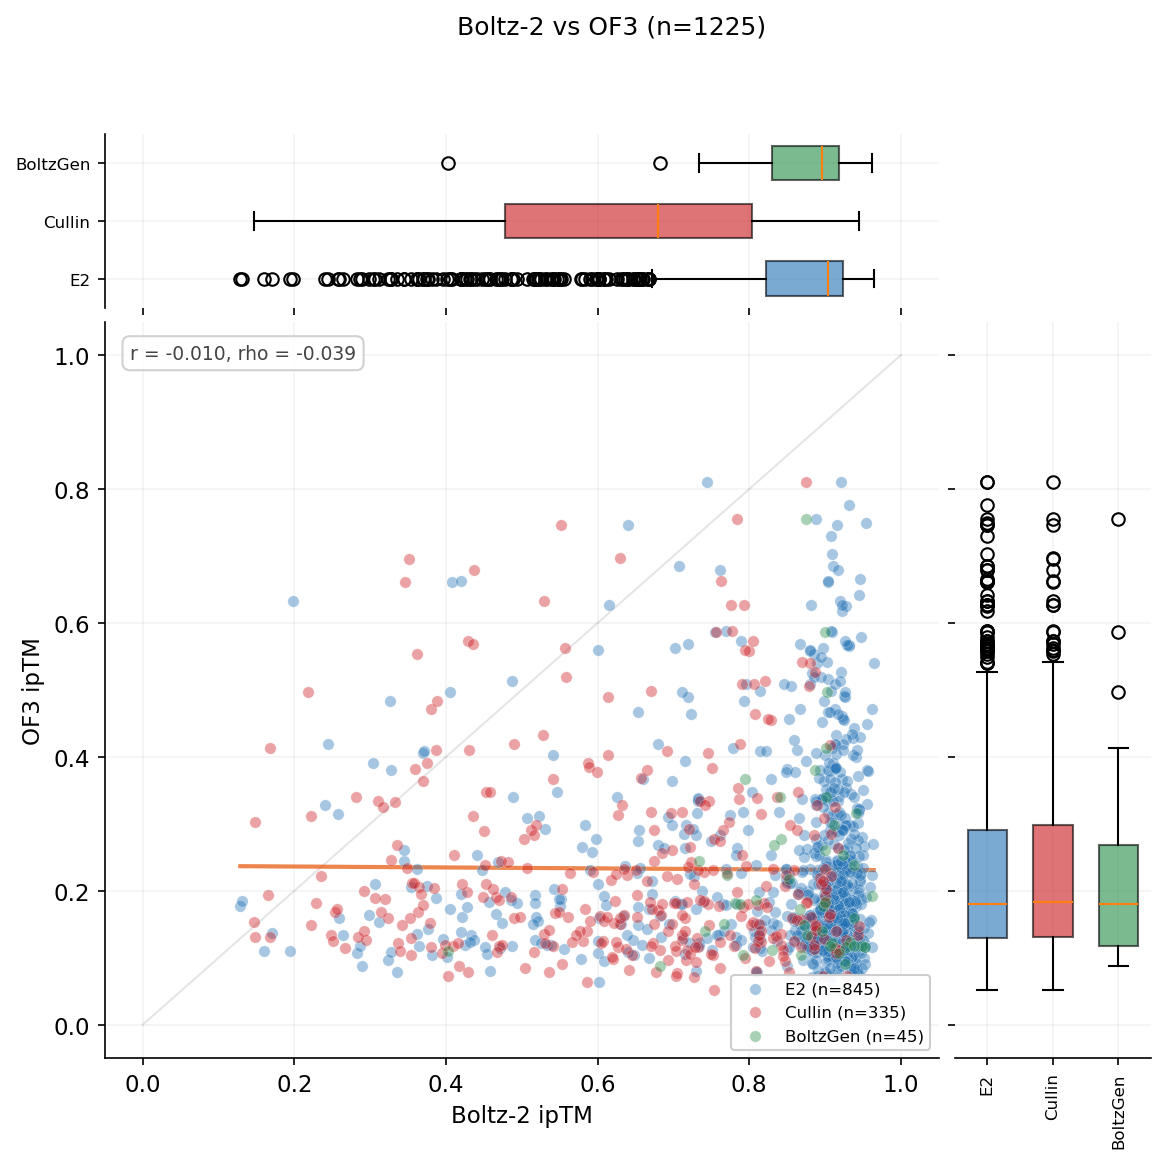
\includegraphics[width=0.85\textwidth]{rbx1_plots/pipe_boltz_vs_of3.png}
\caption{Boltz-2 ipTM vs.\ OpenFold3 ipTM ($n = 1{,}225$). Pearson $r = -0.01$, Spearman $\rho = -0.04$. No correlation.}
\label{fig:boltz_vs_of3}
\end{figure}

%% ============================================================
\section{Top Designs}
%% ============================================================

\subsection{Top 18 by AlphaFold3 ipTM}

Table~\ref{tab:top_af3} lists all designs with AF3 ipTM $\geq 0.50$, ranked by AF3 ipTM. The best design by AF3 is \texttt{wbg\_design\_1817} (AF3 = 0.85), a BoltzGen design.

\begin{longtable}{clp{2cm}ccccccc}
\caption{Top designs ranked by AlphaFold3 ipTM ($\geq 0.50$).}
\label{tab:top_af3} \\
\toprule
\textbf{Rk} & \textbf{ID} & \textbf{Camp.} & \textbf{Len} & \textbf{AF3} & \textbf{AF3 pTM} & \textbf{OF3} & \textbf{Boltz} & \textbf{Pb} & \textbf{Flag} \\
\midrule
\endfirsthead
\toprule
\textbf{Rk} & \textbf{ID} & \textbf{Camp.} & \textbf{Len} & \textbf{AF3} & \textbf{AF3 pTM} & \textbf{OF3} & \textbf{Boltz} & \textbf{Pb} & \textbf{Flag} \\
\midrule
\endhead
1  & wbg\_design\_1817 & BoltzGen & 64 & 0.85 & 0.73 & 0.12 & 0.93 & 0.13 & top hit \\
2  & w2\_design\_0283  & E2 Face  & 49 & 0.84 & 0.67 & 0.75 & 0.95 & 0.71 & top hit \\
3  & w1\_design\_0357  & Cullin   & 60 & 0.78 & 0.67 & 0.15 & 0.94 & 0.69 & promote \\
4  & w2\_design\_1209  & E2 Face  & 65 & 0.77 & 0.69 & 0.75 & 0.92 & 0.81 & top hit \\
5  & w3\_design\_3061  & E2 Face  & 57 & 0.77 & 0.67 & 0.69 & 0.90 & 0.70 & top hit \\
6  & w2\_design\_5499  & E2 Face  & 63 & 0.76 & 0.66 & 0.73 & 0.91 & 0.18 & top hit \\
7  & wbg\_design\_0198 & BoltzGen & 59 & 0.75 & 0.66 & 0.16 & 0.76 & ---  & top hit \\
8  & w3\_design\_1459  & E2 Face  & 65 & 0.74 & 0.66 & 0.78 & 0.93 & 0.76 & top hit \\
9  & w2\_design\_0217  & E2 Face  & 41 & 0.72 & 0.62 & 0.70 & 0.92 & 0.72 & top hit \\
10 & w3\_design\_3538  & E2 Face  & 43 & 0.70 & 0.62 & 0.63 & 0.93 & 0.76 & top hit \\
11 & w2\_design\_1208  & E2 Face  & 65 & 0.70 & 0.64 & 0.59 & 0.91 & ---  & top hit \\
12 & w2\_design\_0743  & E2 Face  & 57 & 0.69 & 0.62 & 0.62 & 0.92 & ---  & promote \\
13 & w2\_design\_4025  & E2 Face  & 64 & 0.69 & 0.63 & 0.70 & 0.91 & ---  & promote \\
14 & w3\_design\_2356  & E2 Face  & 45 & 0.67 & 0.61 & 0.10 & 0.94 & 0.05 & promote \\
15 & w2\_design\_0218  & E2 Face  & 41 & 0.65 & 0.60 & 0.57 & 0.93 & 0.75 & promote \\
16 & w1\_design\_0389  & E2 Face  & 108& 0.63 & 0.67 & 0.27 & 0.89 & 0.69 & promote \\
17 & w2\_design\_6139  & E2 Face  & 41 & 0.63 & 0.59 & 0.64 & 0.94 & 0.11 & promote \\
18 & w2\_design\_8092  & E2 Face  & 50 & 0.62 & 0.59 & 0.68 & 0.91 & ---  & promote \\
\bottomrule
\end{longtable}

\subsection{Top 20 by Competition Pb ipSAE}

Table~\ref{tab:top_pb} lists the 20 highest-scoring designs in the ADAPTYV competition re-scoring.

\begin{longtable}{clp{2cm}ccccccc}
\caption{Top 20 designs ranked by competition Pb ipSAE.}
\label{tab:top_pb} \\
\toprule
\textbf{Rk} & \textbf{ID} & \textbf{Camp.} & \textbf{Len} & \textbf{Pb} & \textbf{AF3} & \textbf{OF3} & \textbf{Boltz} & \textbf{ipSAE} & \textbf{Flag} \\
\midrule
\endfirsthead
\toprule
\textbf{Rk} & \textbf{ID} & \textbf{Camp.} & \textbf{Len} & \textbf{Pb} & \textbf{AF3} & \textbf{OF3} & \textbf{Boltz} & \textbf{ipSAE} & \textbf{Flag} \\
\midrule
\endhead
1  & w3\_design\_3063  & E2 Face  & 57 & 0.83 & 0.31 & 0.81 & 0.92 & 0.73 & discard \\
2  & w2\_design\_1209  & E2 Face  & 65 & 0.81 & 0.77 & 0.75 & 0.92 & 0.73 & top hit \\
3  & wcm\_design\_0709 & Cullin   & 41 & 0.79 & 0.33 & 0.51 & 0.81 & 0.42 & discard \\
4  & w3\_design\_1459  & E2 Face  & 65 & 0.76 & 0.74 & 0.78 & 0.93 & 0.81 & top hit \\
5  & w3\_design\_3538  & E2 Face  & 43 & 0.76 & 0.70 & 0.63 & 0.93 & 0.75 & top hit \\
6  & w2\_design\_0218  & E2 Face  & 41 & 0.75 & 0.65 & 0.57 & 0.93 & 0.67 & promote \\
7  & wbg\_design\_1458 & BoltzGen & 64 & 0.74 & 0.53 & 0.59 & 0.90 & 0.41 & promote \\
8  & w2\_design\_3061  & E2 Face  & 53 & 0.73 & 0.34 & 0.69 & 0.71 & 0.19 & discard \\
9  & w2\_design\_5942  & E2 Face  & 65 & 0.72 & 0.65 & 0.54 & 0.89 & 0.72 & promote \\
10 & w2\_design\_0217  & E2 Face  & 41 & 0.72 & 0.72 & 0.70 & 0.92 & 0.69 & top hit \\
11 & w2\_design\_0283  & E2 Face  & 49 & 0.71 & 0.84 & 0.75 & 0.95 & 0.80 & top hit \\
12 & w2\_design\_0316  & E2 Face  & 41 & 0.71 & ---  & 0.70 & 0.93 & 0.69 & ---     \\
13 & w2\_design\_6225  & E2 Face  & 48 & 0.70 & 0.50 & 0.55 & 0.89 & 0.71 & promote \\
14 & w3\_design\_3061  & E2 Face  & 57 & 0.70 & 0.77 & 0.69 & 0.90 & 0.69 & top hit \\
15 & w2\_design\_5293  & E2 Face  & 57 & 0.70 & 0.63 & 0.56 & 0.88 & 0.68 & promote \\
16 & w1\_design\_0357  & Cullin   & 60 & 0.69 & 0.78 & 0.15 & 0.94 & 0.81 & promote \\
17 & w1\_design\_0389  & E2 Face  & 108& 0.69 & 0.63 & 0.27 & 0.89 & 0.76 & promote \\
18 & w2\_design\_5764  & E2 Face  & 65 & 0.69 & ---  & 0.54 & 0.90 & 0.69 & ---     \\
19 & wcm\_design\_3063 & Cullin   & 43 & 0.68 & 0.24 & 0.81 & 0.87 & 0.59 & discard \\
20 & w2\_design\_1458  & E2 Face  & 50 & 0.68 & 0.41 & 0.59 & 0.75 & 0.43 & review  \\
\bottomrule
\end{longtable}

\subsection{Full Sequences of Top 5 AF3 Designs}

\begin{enumerate}
\item \textbf{wbg\_design\_1817} (AF3 = 0.85, 64 AA, BoltzGen):\\
\texttt{\seqsplit{SAAAAAGEKAAAAAEAGASTDELAKLWVEAAKLAAASSDPAAANAAFIGIAKAIVIRMKRLLGL}}

\item \textbf{w2\_design\_0283} (AF3 = 0.84, 49 AA, E2 Face):\\
\texttt{\seqsplit{LDELMKKLKEELEELREKLREAVKAGDEEKAEELRKRLFDCIIELSKLK}}

\item \textbf{w1\_design\_0357} (AF3 = 0.78, 60 AA, Cullin Face):\\
\texttt{\seqsplit{SRMEENRRARAERAEALRAAGDLAALEALLAAEAAAQAALAAAAERERAERERRRAEEEA}}

\item \textbf{w2\_design\_1209} (AF3 = 0.77, 65 AA, E2 Face):\\
\texttt{\seqsplit{LSEEELEELERERRELEELREELERKIEEAESEEEKKELEKKLEEVEAHIRCLEARELILEAAEP}}

\item \textbf{w2\_design\_5499} (AF3 = 0.76, 63 AA, E2 Face):\\
\texttt{\seqsplit{PKDRKTLEELKKELEERRERAEELLKSPSPSTQSLGKAQLLVCEEAEEKIKKLEEELRKEEEA}}
\end{enumerate}

%% ============================================================
\section{Pipeline Performance}
%% ============================================================

\begin{figure}[H]
\centering
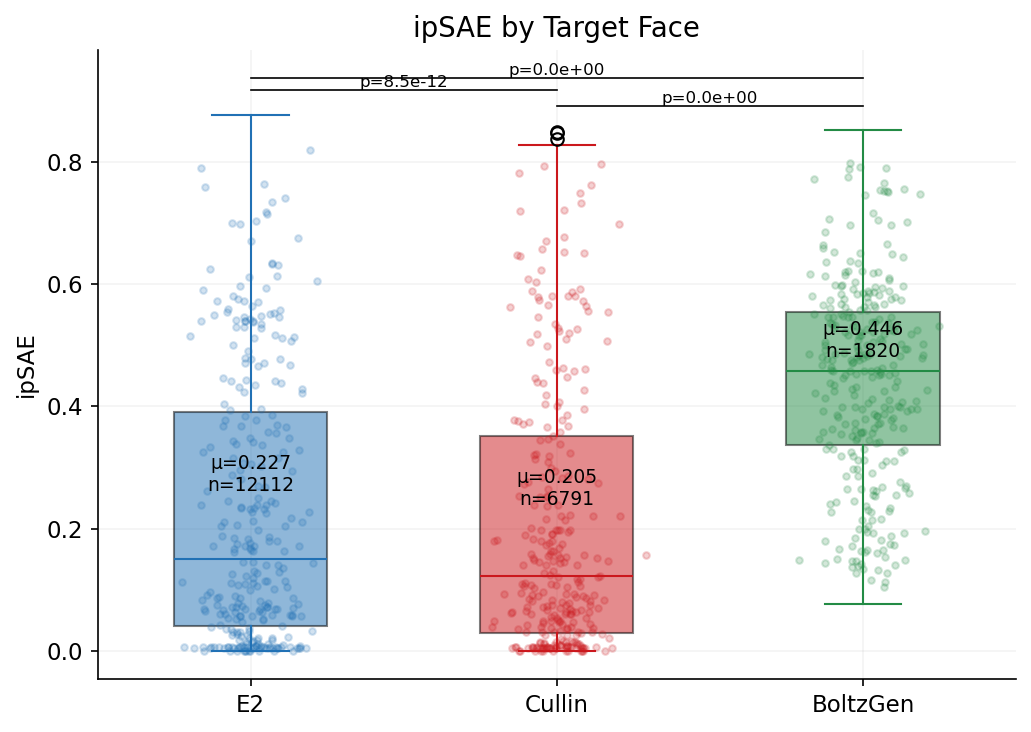
\includegraphics[width=\textwidth]{rbx1_plots/pipe_ipsae_by_face.png}
\caption{ipSAE distribution by target face. BoltzGen designs show inflated ipSAE (mean 0.446) compared to RFdiffusion campaigns (E2: 0.227, Cullin: 0.205).}
\label{fig:ipsae_by_face}
\end{figure}

\begin{figure}[H]
\centering
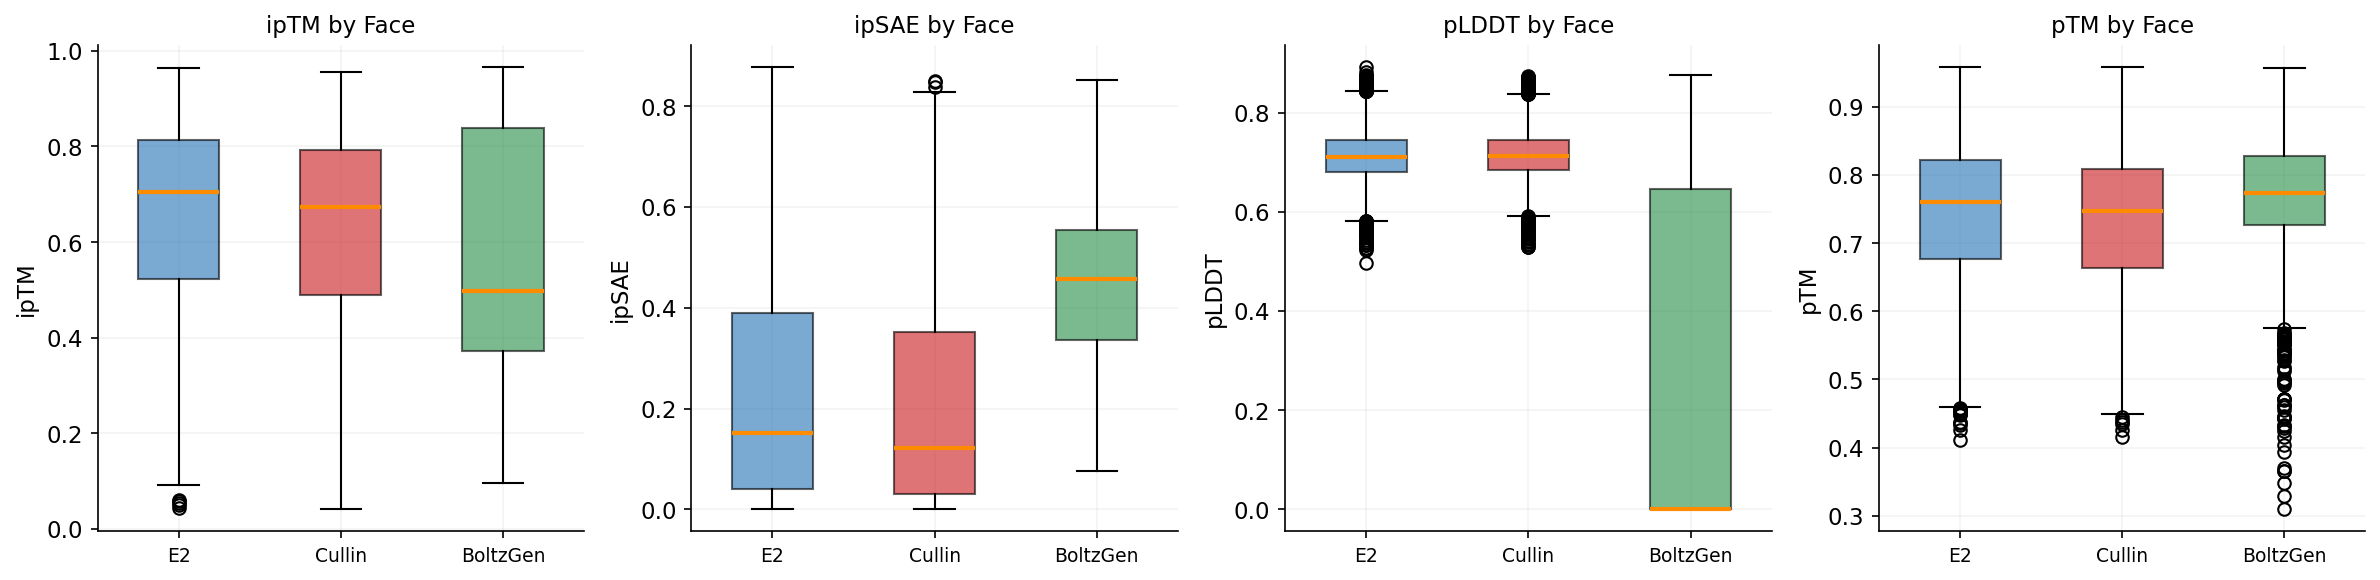
\includegraphics[width=\textwidth]{rbx1_plots/pipe_metrics_by_face.png}
\caption{Multi-metric comparison across target faces and pipeline types.}
\label{fig:metrics_by_face}
\end{figure}

\begin{figure}[H]
\centering
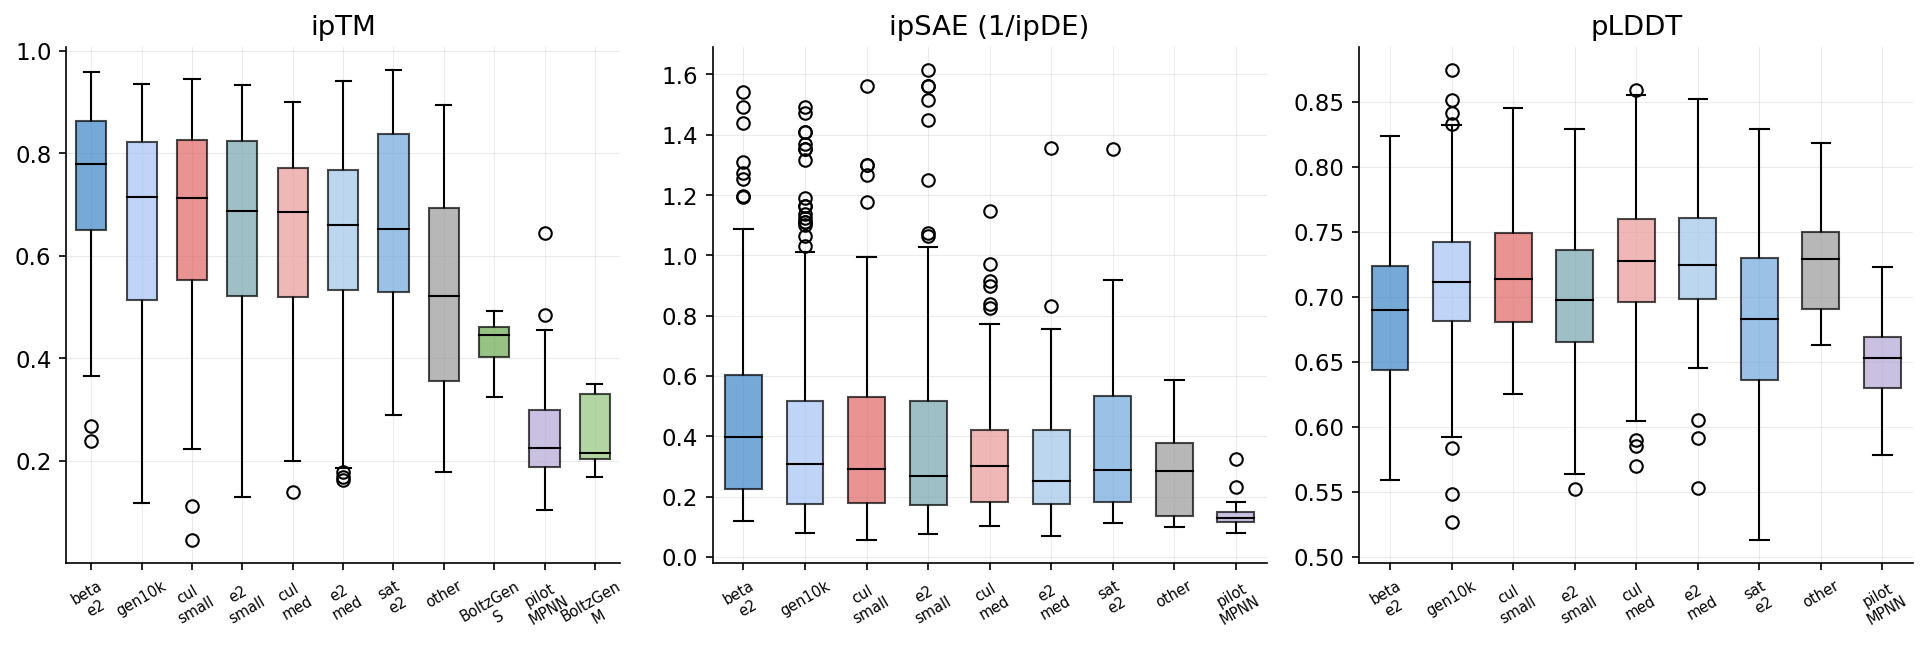
\includegraphics[width=\textwidth]{rbx1_plots/pipeline_comparison.png}
\caption{Side-by-side comparison of Boltz-2, OpenFold3, and AlphaFold3 scores for top designs.}
\label{fig:pipeline_comparison}
\end{figure}

\begin{figure}[H]
\centering
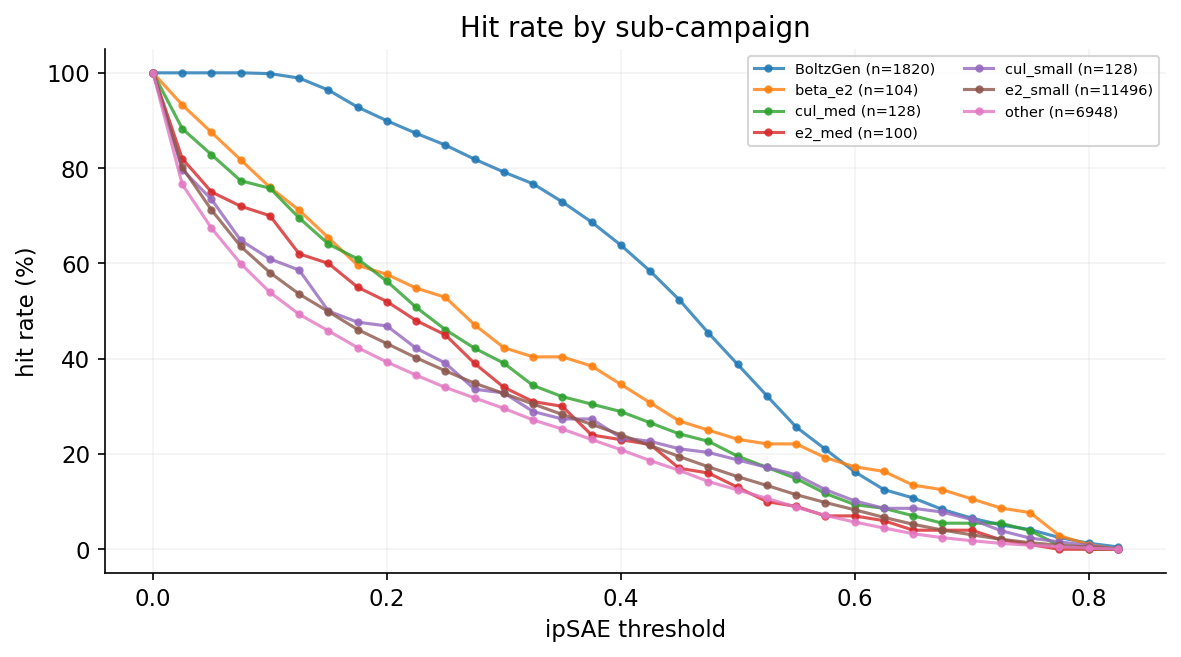
\includegraphics[width=\textwidth]{rbx1_plots/hit_rate_comparison.png}
\caption{Hit rates across scoring methods and campaigns.}
\label{fig:hit_rate}
\end{figure}

\begin{figure}[H]
\centering
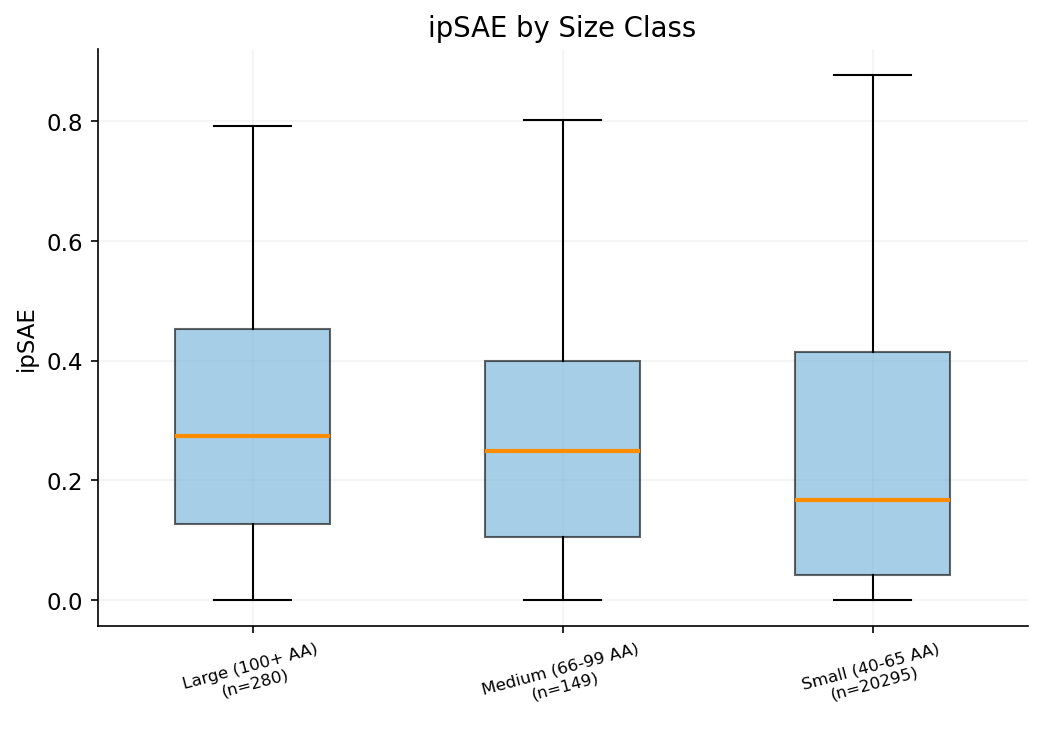
\includegraphics[width=\textwidth]{rbx1_plots/pipe_ipsae_by_size.png}
\caption{ipSAE distribution by binder size class.}
\label{fig:ipsae_by_size}
\end{figure}

%% ============================================================
\section{AlphaFold3 Insights}
%% ============================================================

Comprehensive analysis of what predicts AF3 validation success across 60 validated designs (14 top hits with AF3 ipTM $\geq 0.70$).

\begin{figure}[H]
\centering
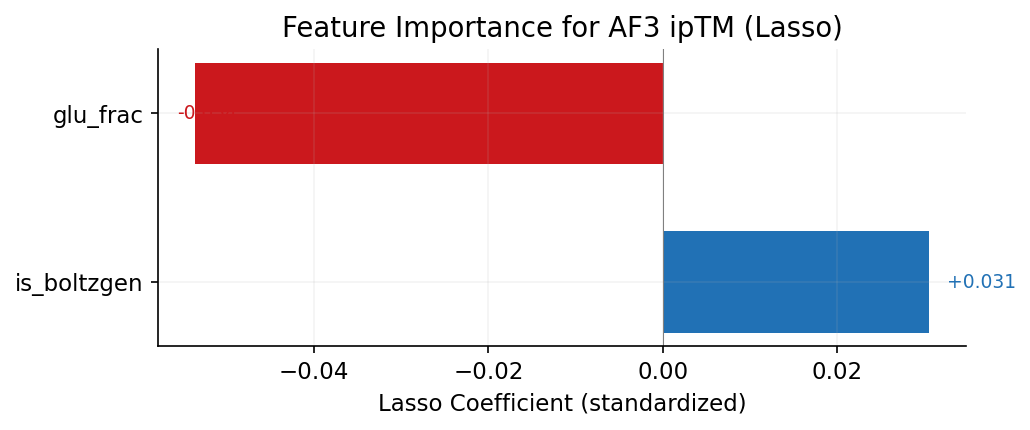
\includegraphics[width=\textwidth]{rbx1_plots/af3_lasso_coefs.png}
\caption{LASSO regression coefficients predicting AF3 ipTM from sequence and structural features. Asp content is the strongest positive predictor; Glu content is negative.}
\label{fig:af3_lasso}
\end{figure}

\begin{figure}[H]
\centering
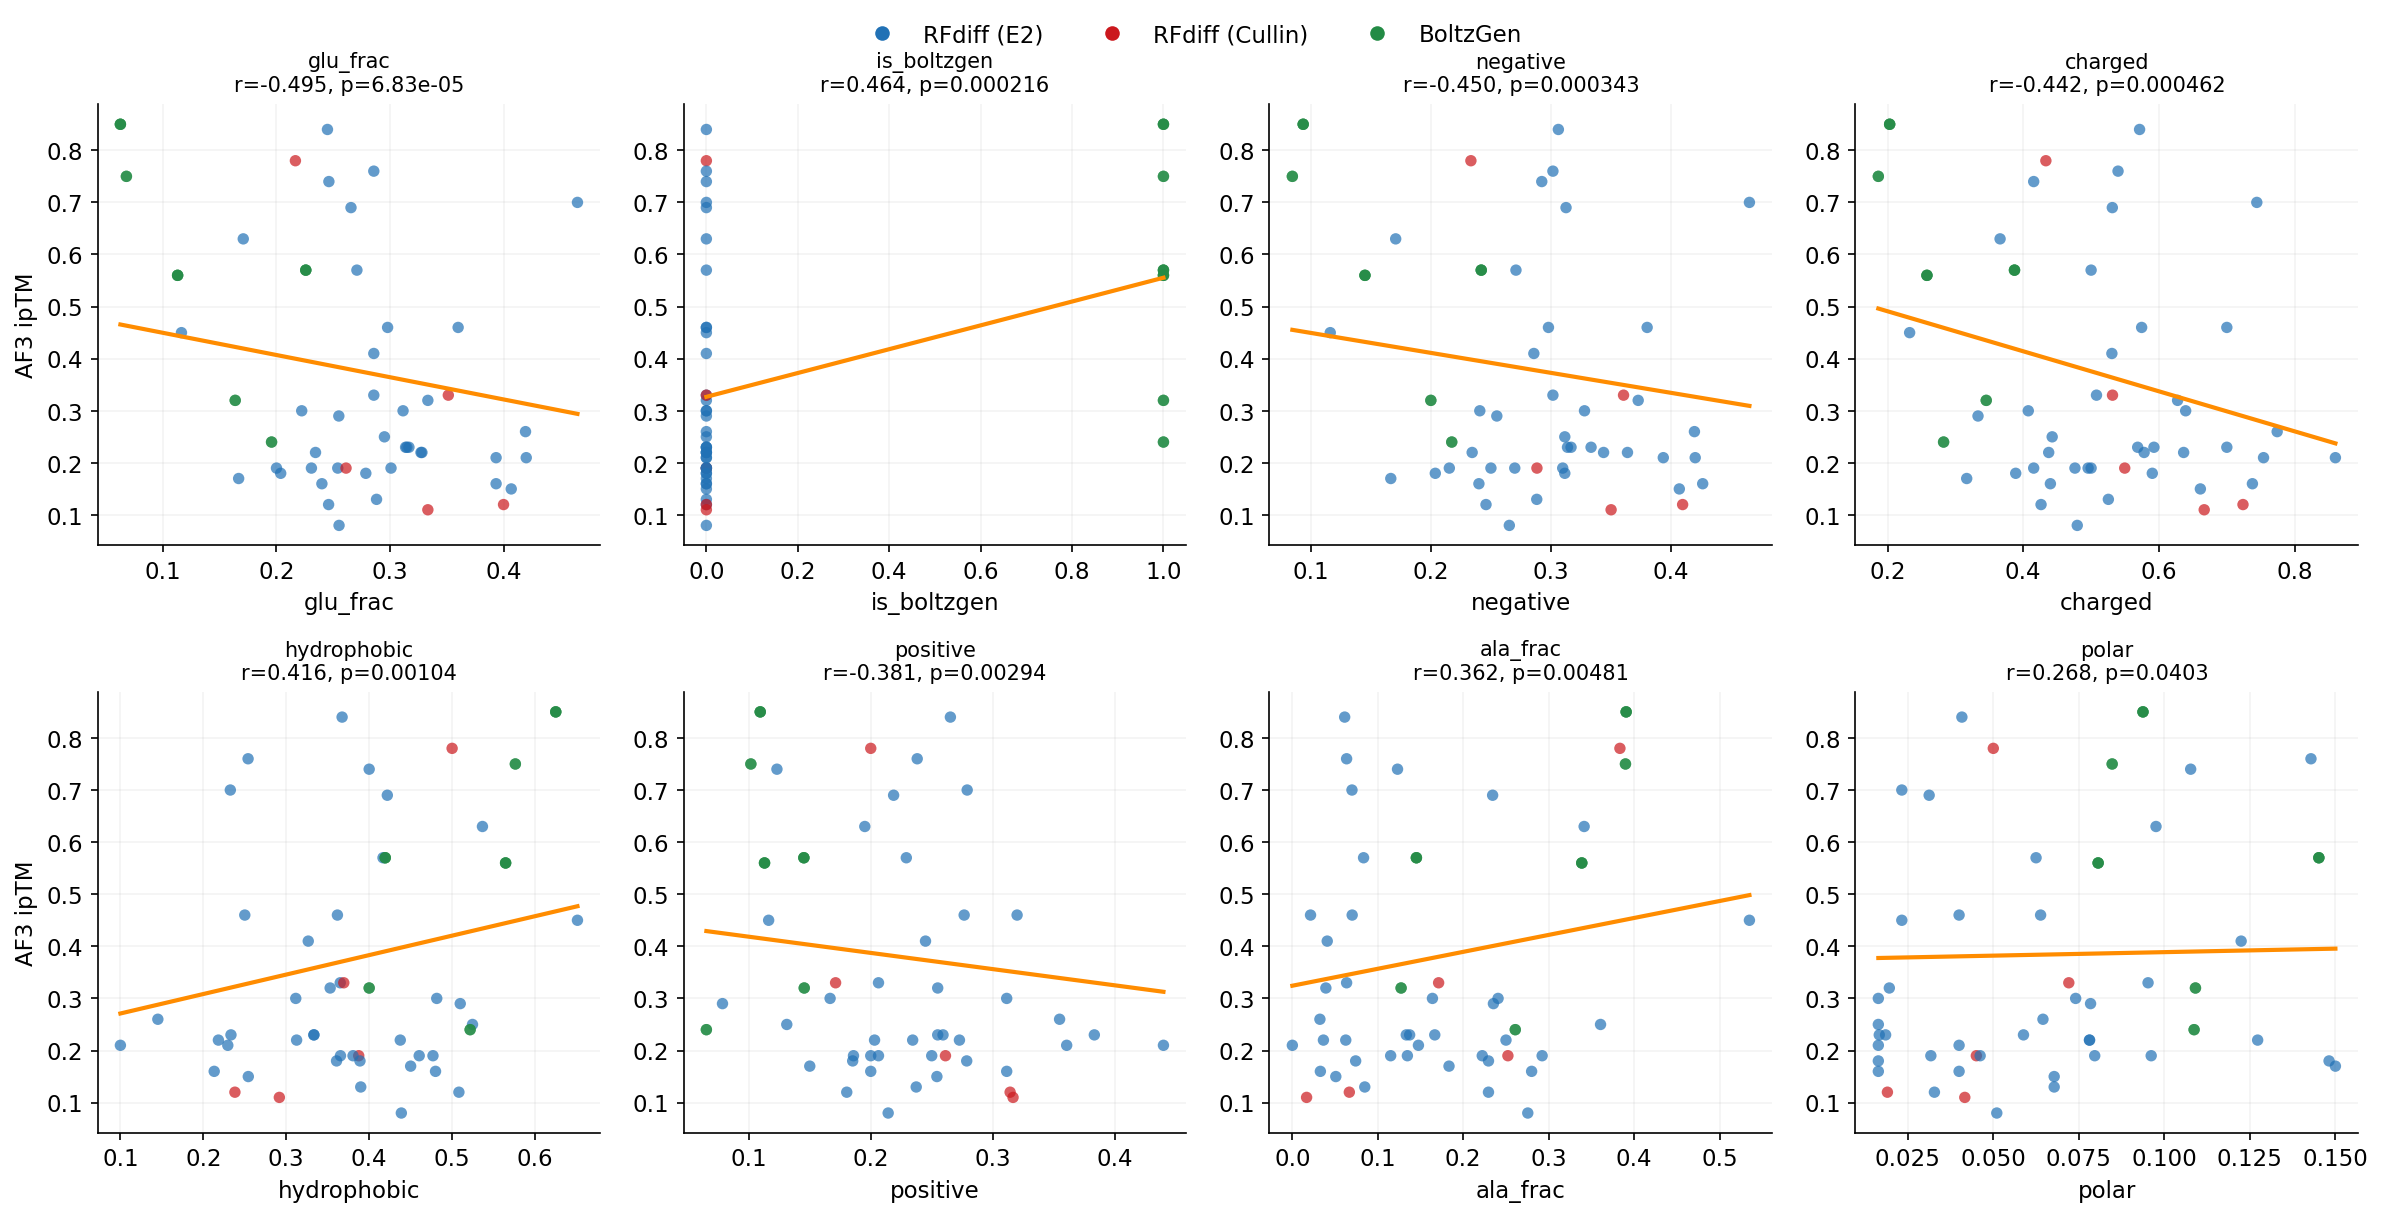
\includegraphics[width=\textwidth]{rbx1_plots/af3_feature_importance.png}
\caption{Random forest feature importance for AF3 ipTM prediction.}
\label{fig:af3_importance}
\end{figure}

\begin{figure}[H]
\centering
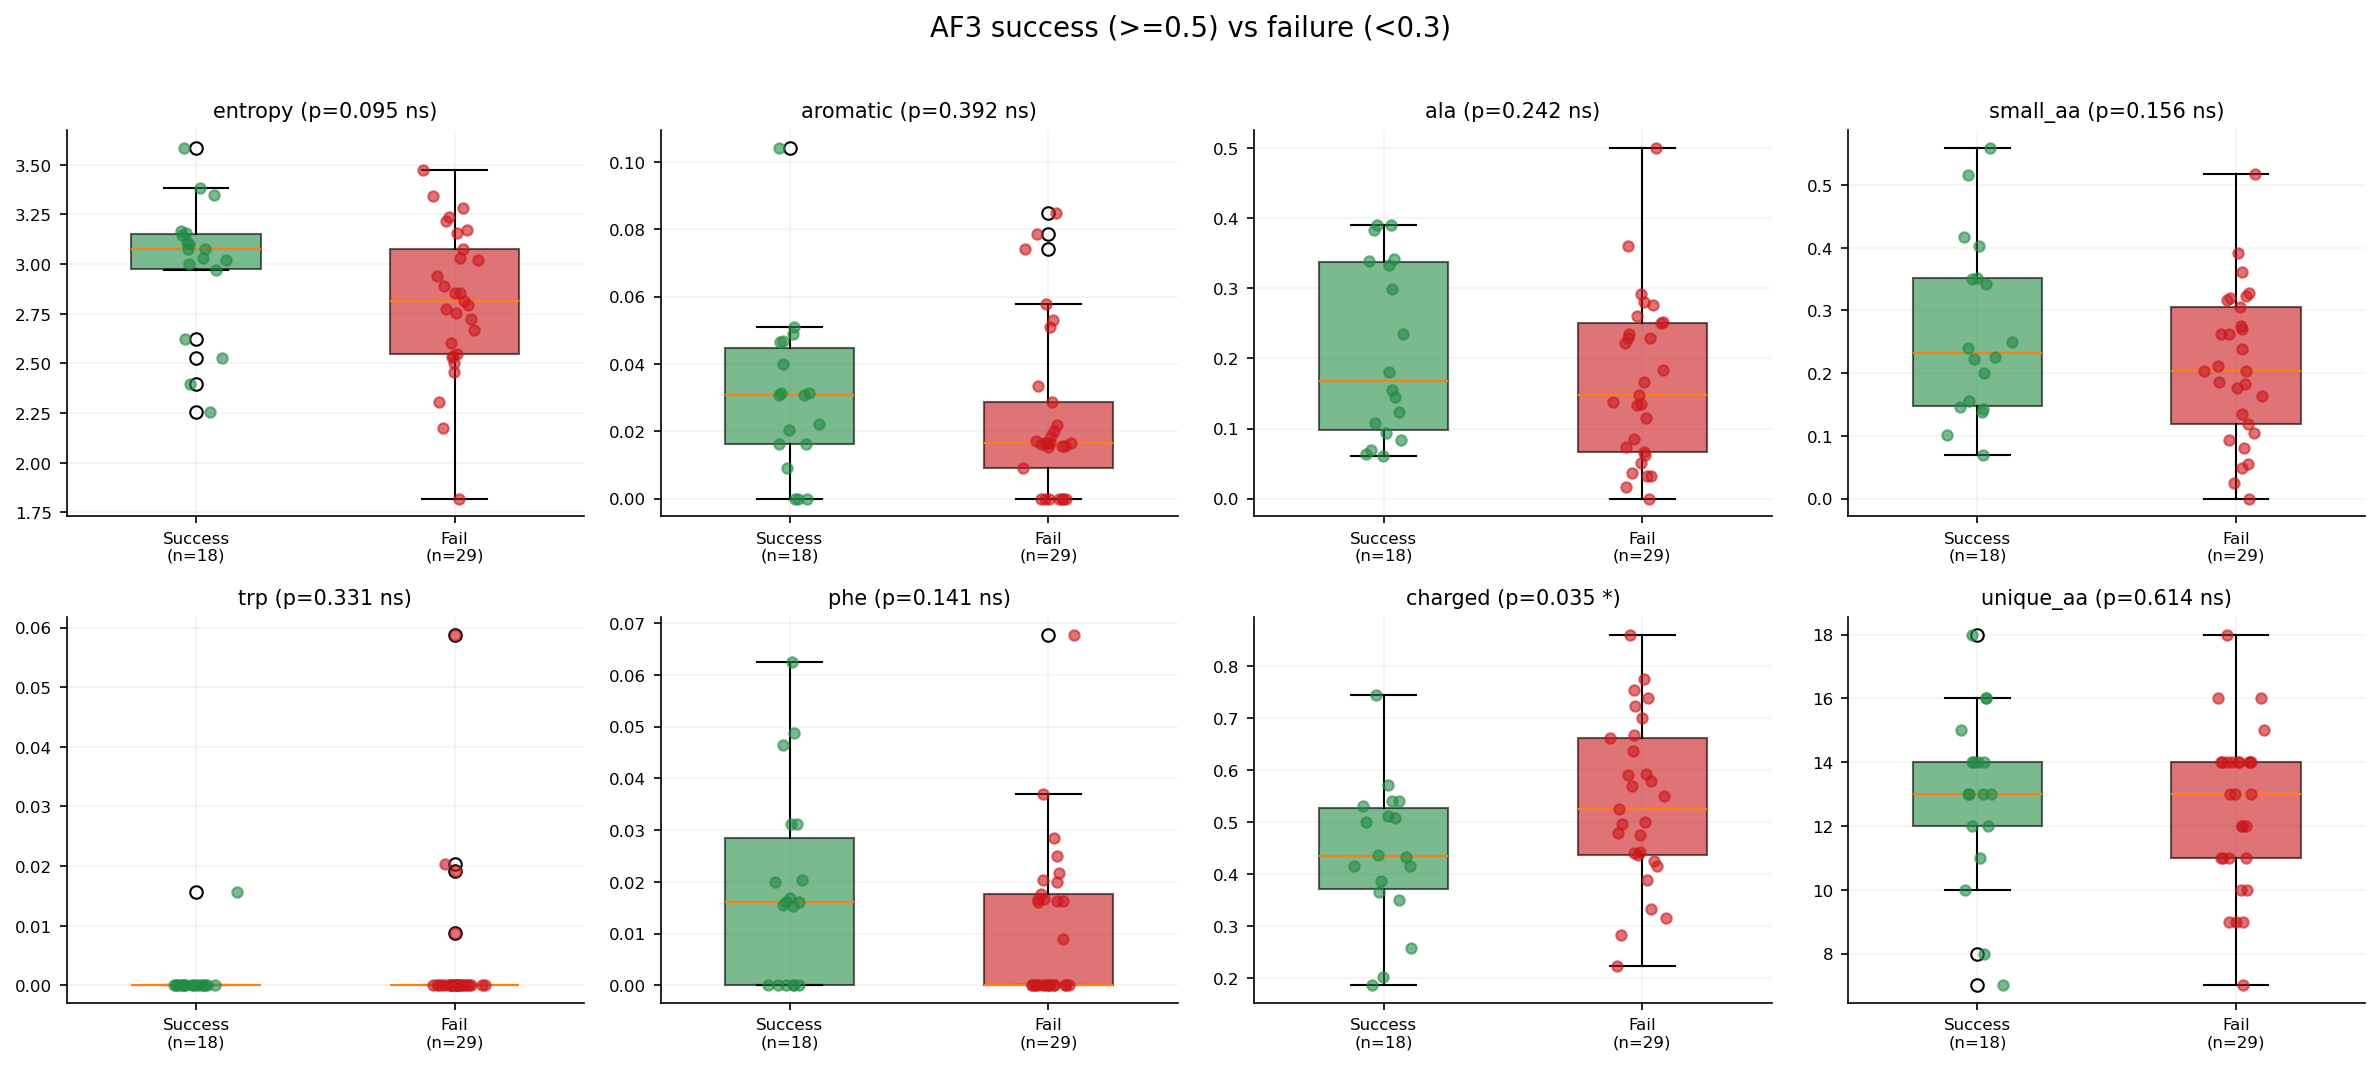
\includegraphics[width=\textwidth]{rbx1_plots/af3_success_vs_fail.png}
\caption{Feature comparison between AF3-successful ($\geq 0.70$) and AF3-failed ($< 0.50$) designs.}
\label{fig:af3_success_fail}
\end{figure}

\begin{figure}[H]
\centering
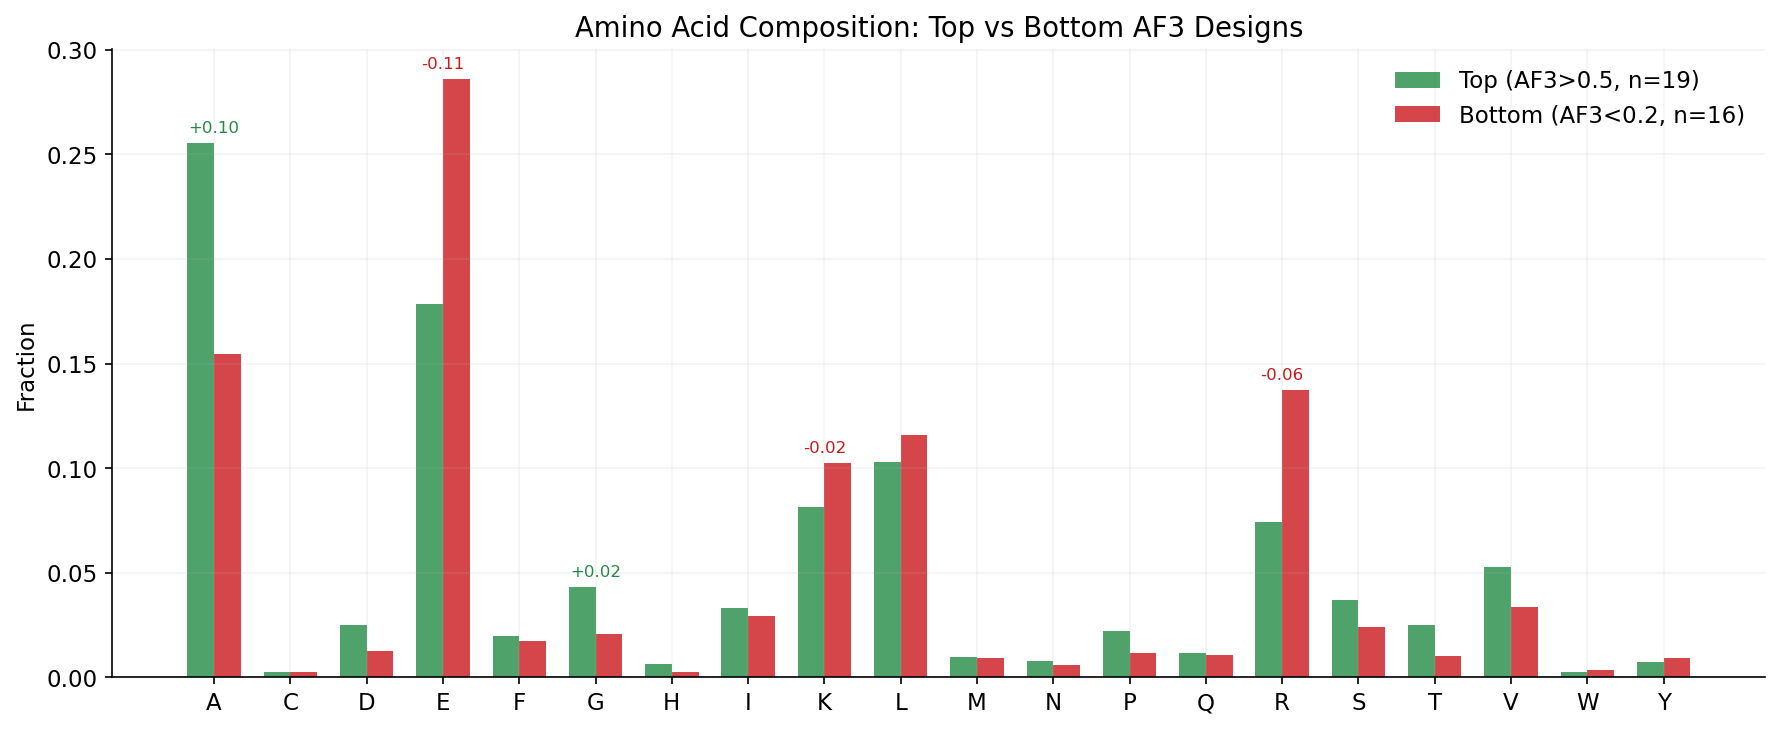
\includegraphics[width=\textwidth]{rbx1_plots/af3_sequence_analysis.png}
\caption{Amino acid composition and sequence-level analysis of AF3-validated designs.}
\label{fig:af3_sequence}
\end{figure}

\begin{figure}[H]
\centering
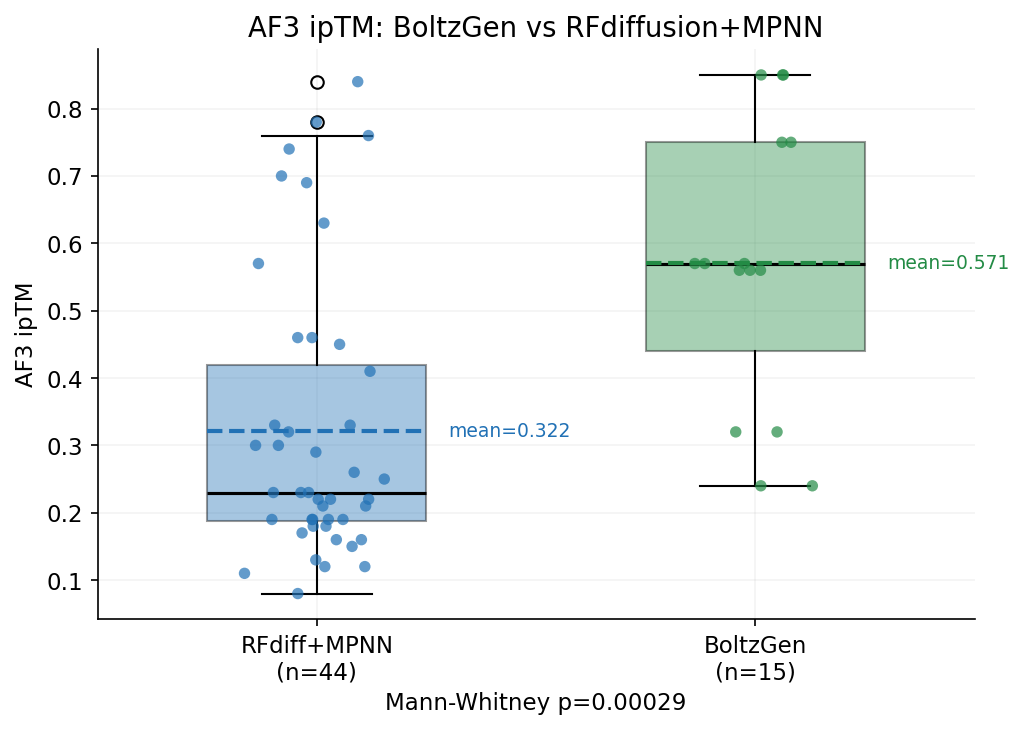
\includegraphics[width=\textwidth]{rbx1_plots/af3_boltzgen_vs_rfdiff.png}
\caption{BoltzGen vs.\ RFdiffusion+MPNN designs in AF3 validation. BoltzGen designs validate at a higher rate despite lower sequence complexity.}
\label{fig:af3_boltzgen}
\end{figure}

Key findings from AF3 analysis:
\begin{itemize}
  \item Aspartate (D) content is the strongest positive predictor of AF3 success.
  \item Glutamate (E) content is negatively associated --- despite E and D being chemically similar.
  \item BoltzGen designs validate at a higher rate than RFdiffusion+MPNN designs.
  \item Shannon entropy and aromatic amino acid content are positively associated with AF3 success.
  \item Boltz-2 ipTM and ipSAE have near-zero predictive power for AF3 outcomes.
\end{itemize}

%% ============================================================
\section{Post-Submission Analysis}
%% ============================================================

After submitting 81 designs to the ADAPTYV competition, the organizers independently re-scored all designs with their own Boltz-2 setup. Of 81 submitted, 33 survived (ipSAE $\geq 0.6$) and 31 failed (ipSAE $< 0.3$).

\begin{figure}[H]
\centering
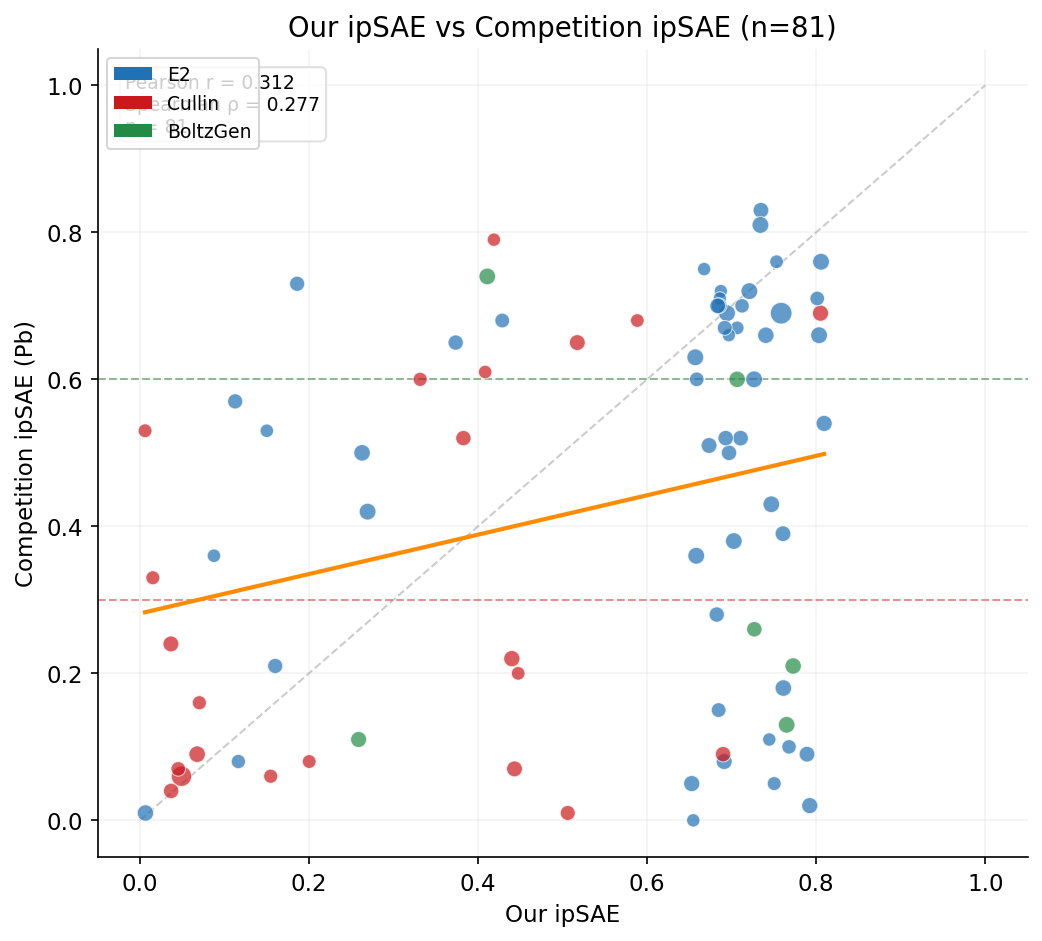
\includegraphics[width=0.85\textwidth]{rbx1_plots/post_our_vs_their_ipsae.png}
\caption{Our ipSAE vs.\ competition ipSAE. Notable reversals: 7 designs we scored below 0.5 survived in competition ($\geq 0.6$), while 9 designs we scored above 0.7 failed ($< 0.3$).}
\label{fig:our_vs_their}
\end{figure}

\begin{figure}[H]
\centering
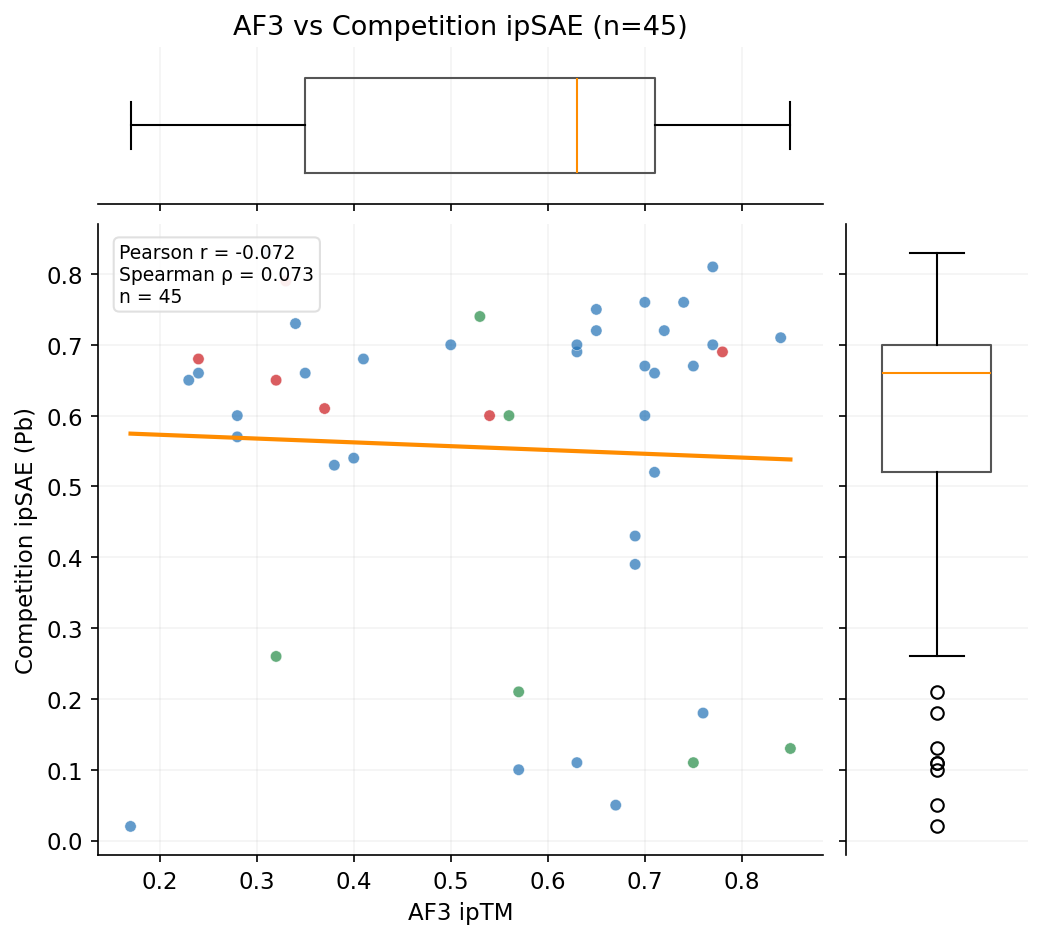
\includegraphics[width=0.85\textwidth]{rbx1_plots/post_af3_vs_pb_ipsae.png}
\caption{AF3 ipTM vs.\ competition Pb ipSAE for designs with both scores.}
\label{fig:af3_vs_pb}
\end{figure}

\begin{figure}[H]
\centering
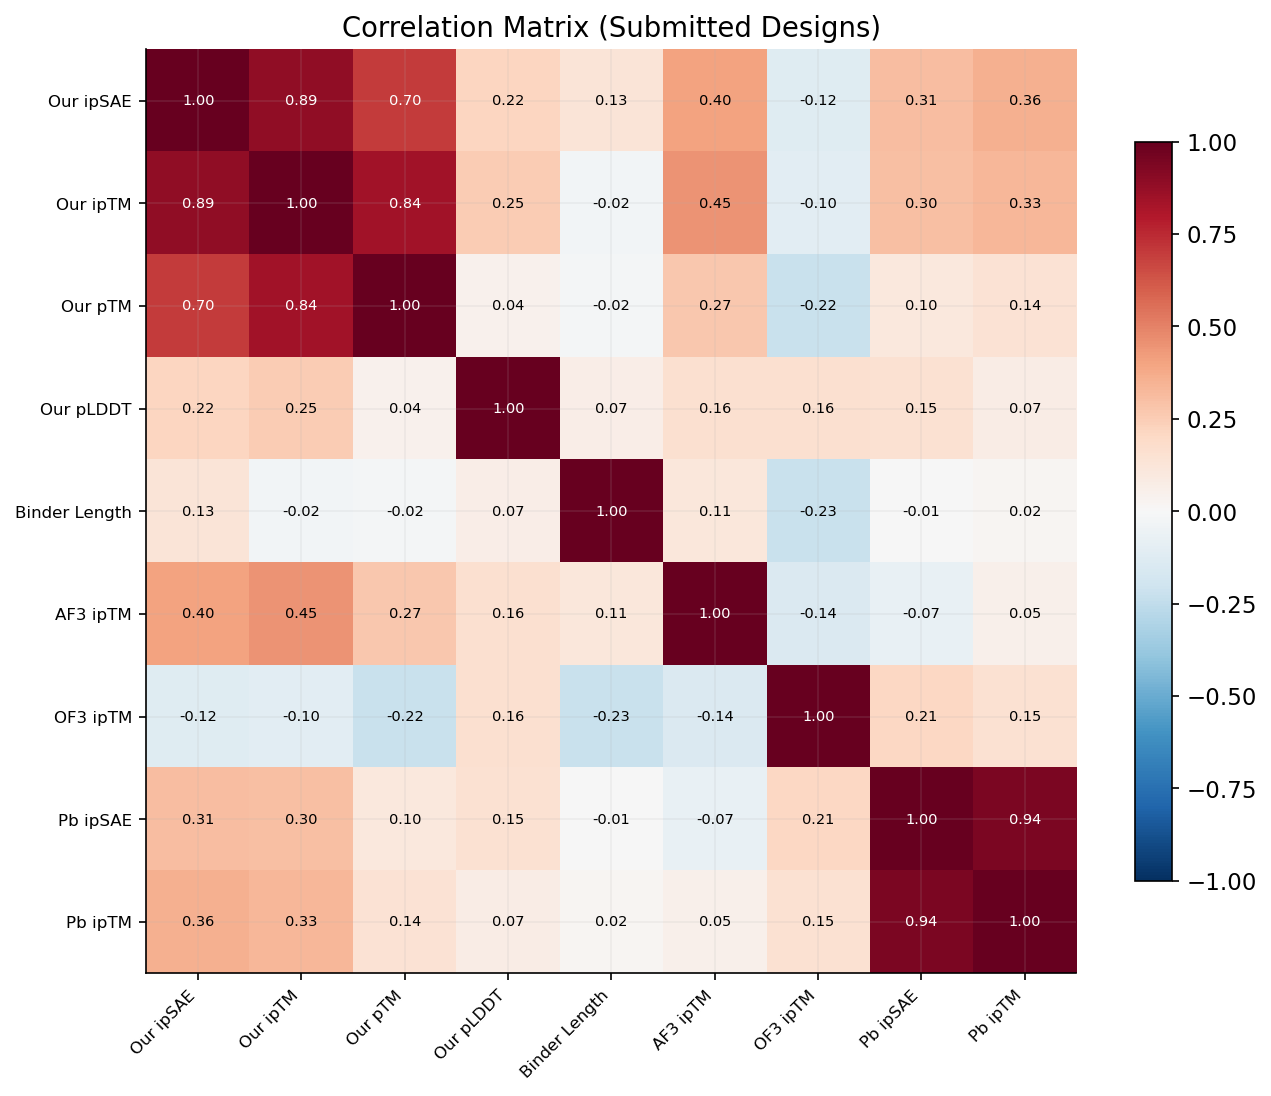
\includegraphics[width=\textwidth]{rbx1_plots/post_full_correlation.png}
\caption{Full correlation matrix of our features vs.\ competition metrics. Competition metrics cluster separately from our pipeline metrics. Charge features show moderate associations with competition outcomes.}
\label{fig:full_corr}
\end{figure}

\begin{figure}[H]
\centering
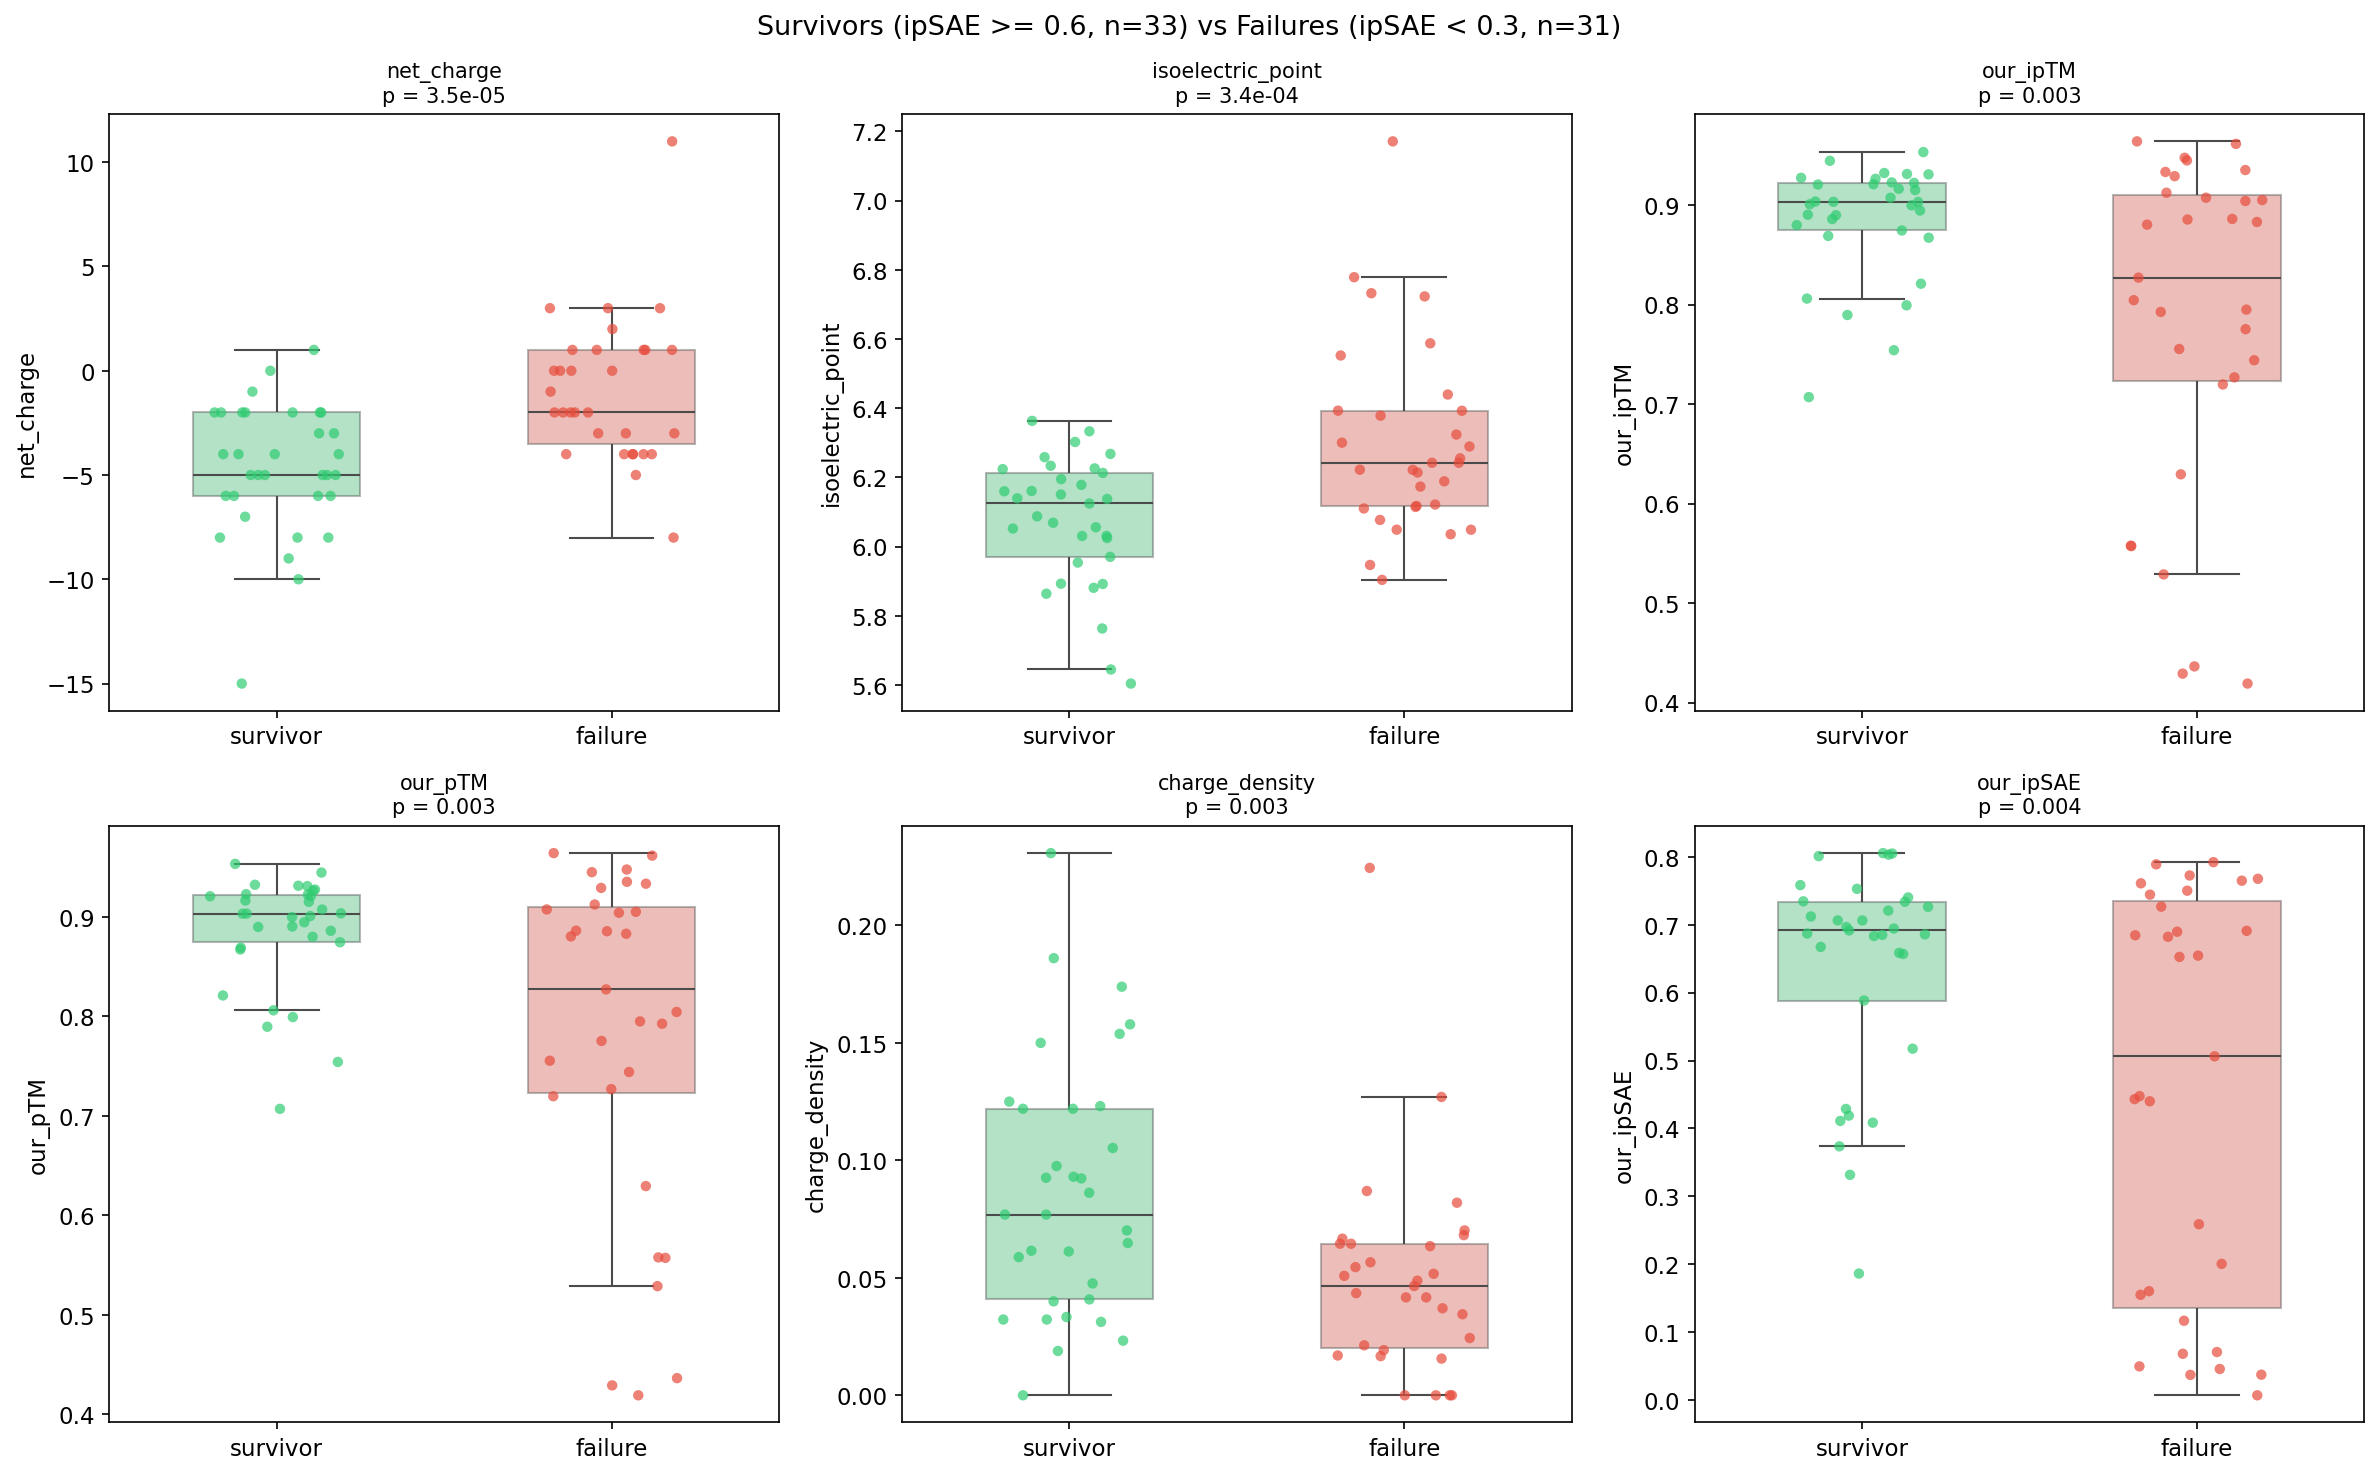
\includegraphics[width=\textwidth]{rbx1_plots/post_survivors_vs_failures.png}
\caption{Feature comparison between competition survivors ($\geq 0.6$) and failures ($< 0.3$).}
\label{fig:survivors_vs_failures}
\end{figure}

\begin{figure}[H]
\centering
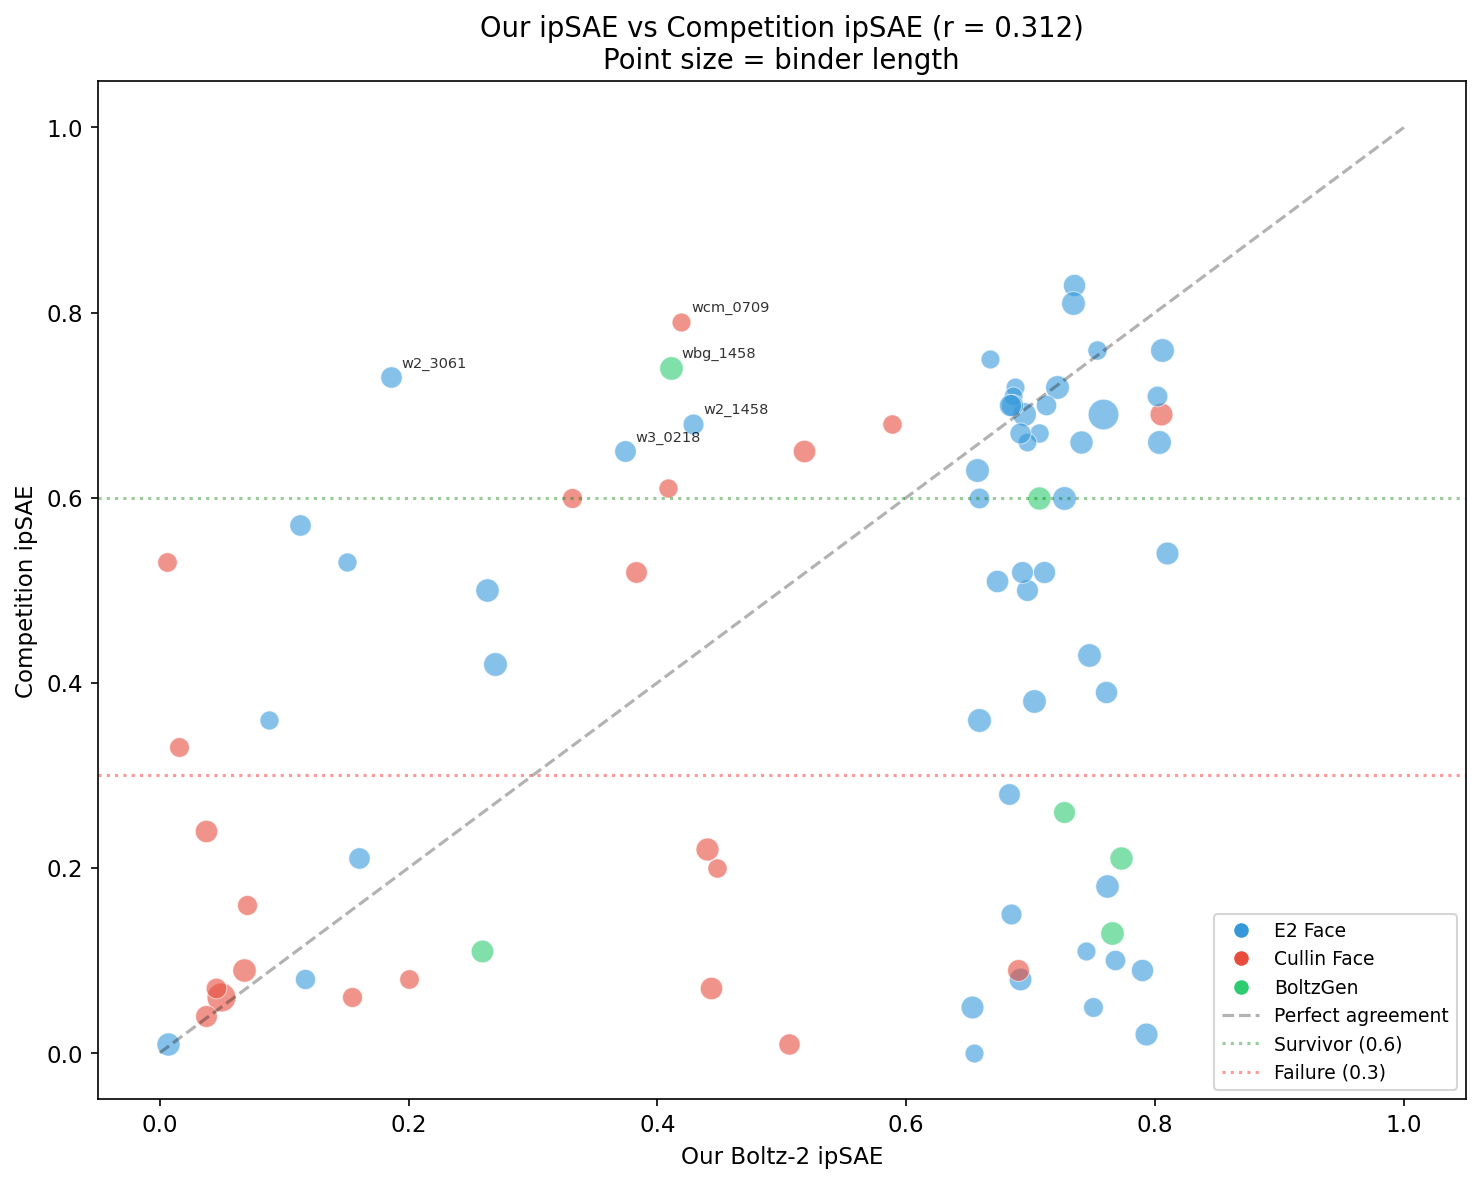
\includegraphics[width=\textwidth]{rbx1_plots/post_submission_overview.png}
\caption{Overview of submission outcomes across all 81 designs.}
\label{fig:submission_overview}
\end{figure}

\subsection{Predictive Modeling of Competition Scores}

Three regression models were trained to predict competition ipSAE from 64 sequence/structural features. All showed \textbf{negative cross-validated $R^2$}, confirming that competition scores are inherently unpredictable from our pipeline features:

\begin{table}[H]
\centering
\caption{Cross-validated $R^2$ for competition ipSAE prediction.}
\begin{tabular}{lc}
\toprule
\textbf{Model} & \textbf{CV $R^2$} \\
\midrule
Ridge Regression     & $-2.22$ \\
ElasticNet           & $-0.69$ \\
Random Forest        & $-0.33$ \\
\bottomrule
\end{tabular}
\end{table}

The top discriminating features between survivors and failures (Mann--Whitney U test):

\begin{table}[H]
\centering
\caption{Top features discriminating competition survivors vs.\ failures.}
\begin{tabular}{lcc}
\toprule
\textbf{Feature} & \textbf{$p$-value} & \textbf{Importance (RF)} \\
\midrule
Net charge         & $3.5 \times 10^{-5}$ & 0.105 \\
Isoelectric point  & $3.4 \times 10^{-4}$ & 0.074 \\
Our ipTM           & $3.0 \times 10^{-3}$ & ---   \\
Charge density     & $3.2 \times 10^{-3}$ & 0.066 \\
Our ipSAE          & $3.9 \times 10^{-3}$ & 0.041 \\
Serine content     & ---                   & 0.083 \\
\bottomrule
\end{tabular}
\end{table}

\textbf{Net charge is the single strongest predictor of competition survival.} The competition likely uses a fine-tuned or differently-configured Boltz-2 that is sensitive to electrostatic properties not captured by our scoring setup.

%% ============================================================
\section{Evolutionary Analysis}
%% ============================================================

ESM-2 deep mutational scanning (DMS) was performed on 2,160 single-point mutations across the 108-residue RBX1 target.

Key findings:
\begin{itemize}
  \item Conservation (from 165-sequence MSA) correlates with ESM-2 DMS sensitivity (Spearman $r = 0.58$).
  \item Zinc-coordinating cysteines and histidines dominate both conservation and DMS sensitivity profiles.
  \item DMS-guided hotspot selection (E2 Enhanced) produced the highest AF3 hit rate among RFdiffusion campaigns.
\end{itemize}

%% ============================================================
\section{Conclusions and Future Directions}
%% ============================================================

\subsection{Key Conclusions}

\begin{enumerate}
  \item \textbf{Boltz-2 scoring is unreliable as a filter.} ipSAE and ipTM show near-zero correlation with AF3 ground truth ($r \leq 0.08$). E2-face designs show systematically inflated Boltz-2 scores.
  \item \textbf{AlphaFold3 is the reliable ground truth.} AF3 ipTM is the most trustworthy metric; OF3 shows moderate agreement ($r = 0.57$).
  \item \textbf{Sequence diversity predicts AF3 success.} Shannon entropy, aromatic content, and Asp fraction are positive predictors; low-complexity poly-Ala/Glu sequences fail.
  \item \textbf{Competition scoring is unpredictable.} The ADAPTYV Boltz-2 re-scoring produces results that are only weakly correlated with our scores ($r = 0.31$) and show dramatic reversals. Net charge is the strongest (but still weak) predictor.
  \item \textbf{BoltzGen is a viable alternative.} Despite generating simpler sequences, BoltzGen designs validate at a higher rate in AF3.
\end{enumerate}

\subsection{Recommendations for Future Campaigns}

\begin{itemize}
  \item Use AF3 (or OF3 as a proxy) for all final design selection --- do not rely on Boltz-2 scores alone.
  \item Optimize for sequence diversity: penalize low-entropy, poly-charged sequences.
  \item Incorporate net charge and isoelectric point as design filters if targeting Boltz-2-based competitions.
  \item Expand BoltzGen sampling, which shows promise for generating AF3-validated binders.
  \item Explore ensemble scoring (Boltz-2 + OF3 + AF3) for more robust design ranking.
\end{itemize}

%% ============================================================
\appendix
\section{Design Naming Convention}
%% ============================================================

Design identifiers follow the pattern \texttt{<wave>\_design\_<number>}:

\begin{itemize}
  \item \texttt{w1}: Wave 1 --- Cullin-face RFdiffusion designs.
  \item \texttt{w2}: Wave 2 --- E2-face RFdiffusion designs (primary campaign).
  \item \texttt{w3}: Wave 3 --- E2-face RFdiffusion designs (enhanced hotspots).
  \item \texttt{wcm}: Cullin-face mass generation wave.
  \item \texttt{wbg}: BoltzGen-generated designs.
  \item \texttt{bg\_small\_*}: Early BoltzGen prototypes.
\end{itemize}

%% ============================================================
\section{Top 100 Design Reference}
%% ============================================================

The full top 100 candidate sequences (ranked by combined OF3/AF3 metrics) are available for download:

\begin{itemize}
  \item FASTA: \texttt{data/rbx1\_top100.fasta}
  \item CSV (all metrics): \texttt{data/rbx1\_top100.csv}
  \item Interactive dashboard: \url{https://sermare.github.io/protein-design.html}
\end{itemize}

\end{document}
